\chapter{Experiments}


\section{Data Collection}
To train our CycleGAN model effectively, we collected a diverse dataset of manga images. We amassed a total of 53GB of data, consisting of 20GB of black and white images and 30GB of colored images in .cbz (Comic Book Zip) format. Each category comprised approximately 100 volumes, ensuring a balanced representation of both monochrome and colored styles.
To ensure consistent colorization results across our dataset and avoid issues arising from disparate artistic styles, we made the deliberate decision to utilize manga images exclusively from the series "One Piece" for training our Cycle-GAN model. \\
This choice was driven by several key factors:
\begin{itemize}
 \item \textbf{Uniform Art Style:}One Piece maintains a remarkable level of artistic consistency throughout its extensive volume count. This consistency provides the model with a well-defined framework for learning color palettes, shading techniques, and character depictions, ultimately leading to more faithful and visually unified colorization outputs.

\item \textbf{Data Abundance:} One Piece boasts a vast wealth of training data, encompassing hundreds of chapters across diverse settings, characters, and emotional portrayals. This abundance allows the model to acquire a comprehensive understanding of the series' overall color scheme and apply it effectively to unseen images.
\end{itemize}

However, it is crucial to acknowledge the potential limitations associated with this data selection:
\begin{itemize}
\item \textbf{Generalizability:}
Restricting the data to a single series may limit the model's ability to generalize effectively to other manga styles. Future exploration of transfer learning techniques could potentially address this limitation.
\item \textbf{Data Bias:} Utilizing solely One Piece introduces potential biases based on the specific color choices and techniques employed within that series. Diversifying the dataset in the future could help mitigate this issue.
\end{itemize}
\newpage

 

\section{Data Preprocessing}

To ensure the effectiveness of our CycleGAN model in colorizing manga images, we implemented a comprehensive data preprocessing pipeline specifically tailored to "One Piece" dataset. This process aimed to refine the raw dataset and provide the model with high-quality, consistent training material.

\subsection{CBZ Extraction and Conversion}

The initial step involved converting all collected CBZ files into individual PNG images. This conversion ensured compatibility with our Networks which accept images as inputs.

\subsection{Page Filtering}

For filtering at high level, we addressed the presence of RGB images in the dataset such as RGB cover pages, end pages, and special trivia and informative pages in the manga.

By effectively removing these colored pages, we ensured the model exclusively learned from black and white manga panels, preventing potential colorization inconsistencies arising from pre-colored content.

\subsection{Panel Detection and Classification}

Subsequently, we addressed the presence of non-manga pages \ref{fig:bad_images} within the dataset which typically are:
\begin{itemize}
    \item Empty pages
    \item Text-only or heavily text-biased pages
    \item Trivia and other non-manga-panel pages
\end{itemize}

To efficiently filter out these non-relevant pages, we employed a Sequential  Convolutional Neural Network (CNN) classifier featuring three 2D convolutional layers followed by max-pooling layers, then flattened and connected to two dense layers for classification. \\This classifier which has architecture as in figure \ref{fig:classifier} was trained on 69 bad manga panels and 900 good manga panels, with Precision: 0.9775, Recall: 1.0, Accuracy: 0.9797 on Validation data on 50 epochs of training.\\
With this CNN classifier, we could systematically identify and remove such non-manga pages from our dataset, ensuring that only relevant content was retained for further processing and analysis.

\begin{figure}[hp]
  \centering
  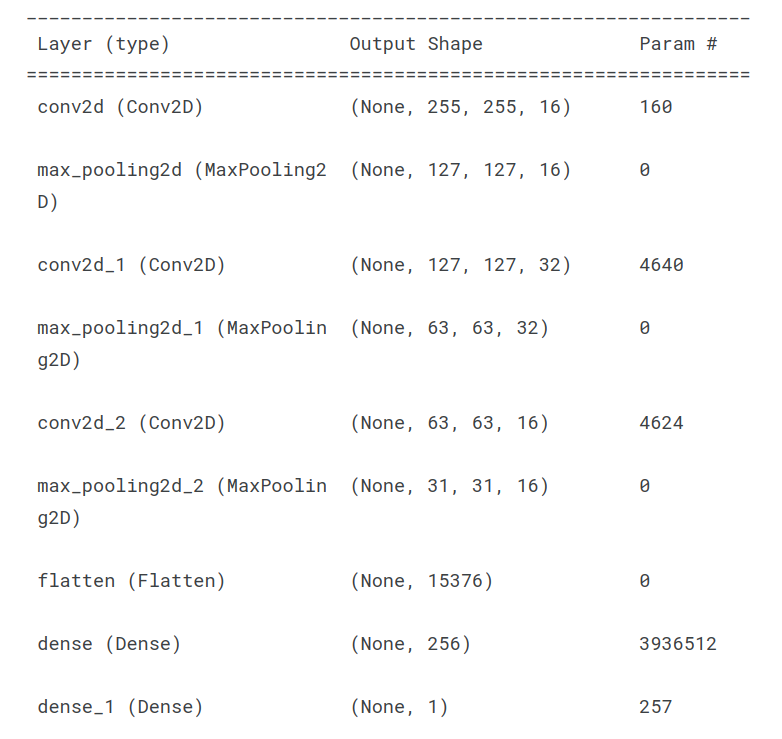
\includegraphics[width=1\textwidth]{chapter/output/classifier-summary.png}
  \caption{Architecture of Manga panel classifier}
  \label{fig:classifier}
\end{figure}


\begin{figure}[htbp]
    \centering
    \begin{subfigure}[b]{0.25\textwidth}
        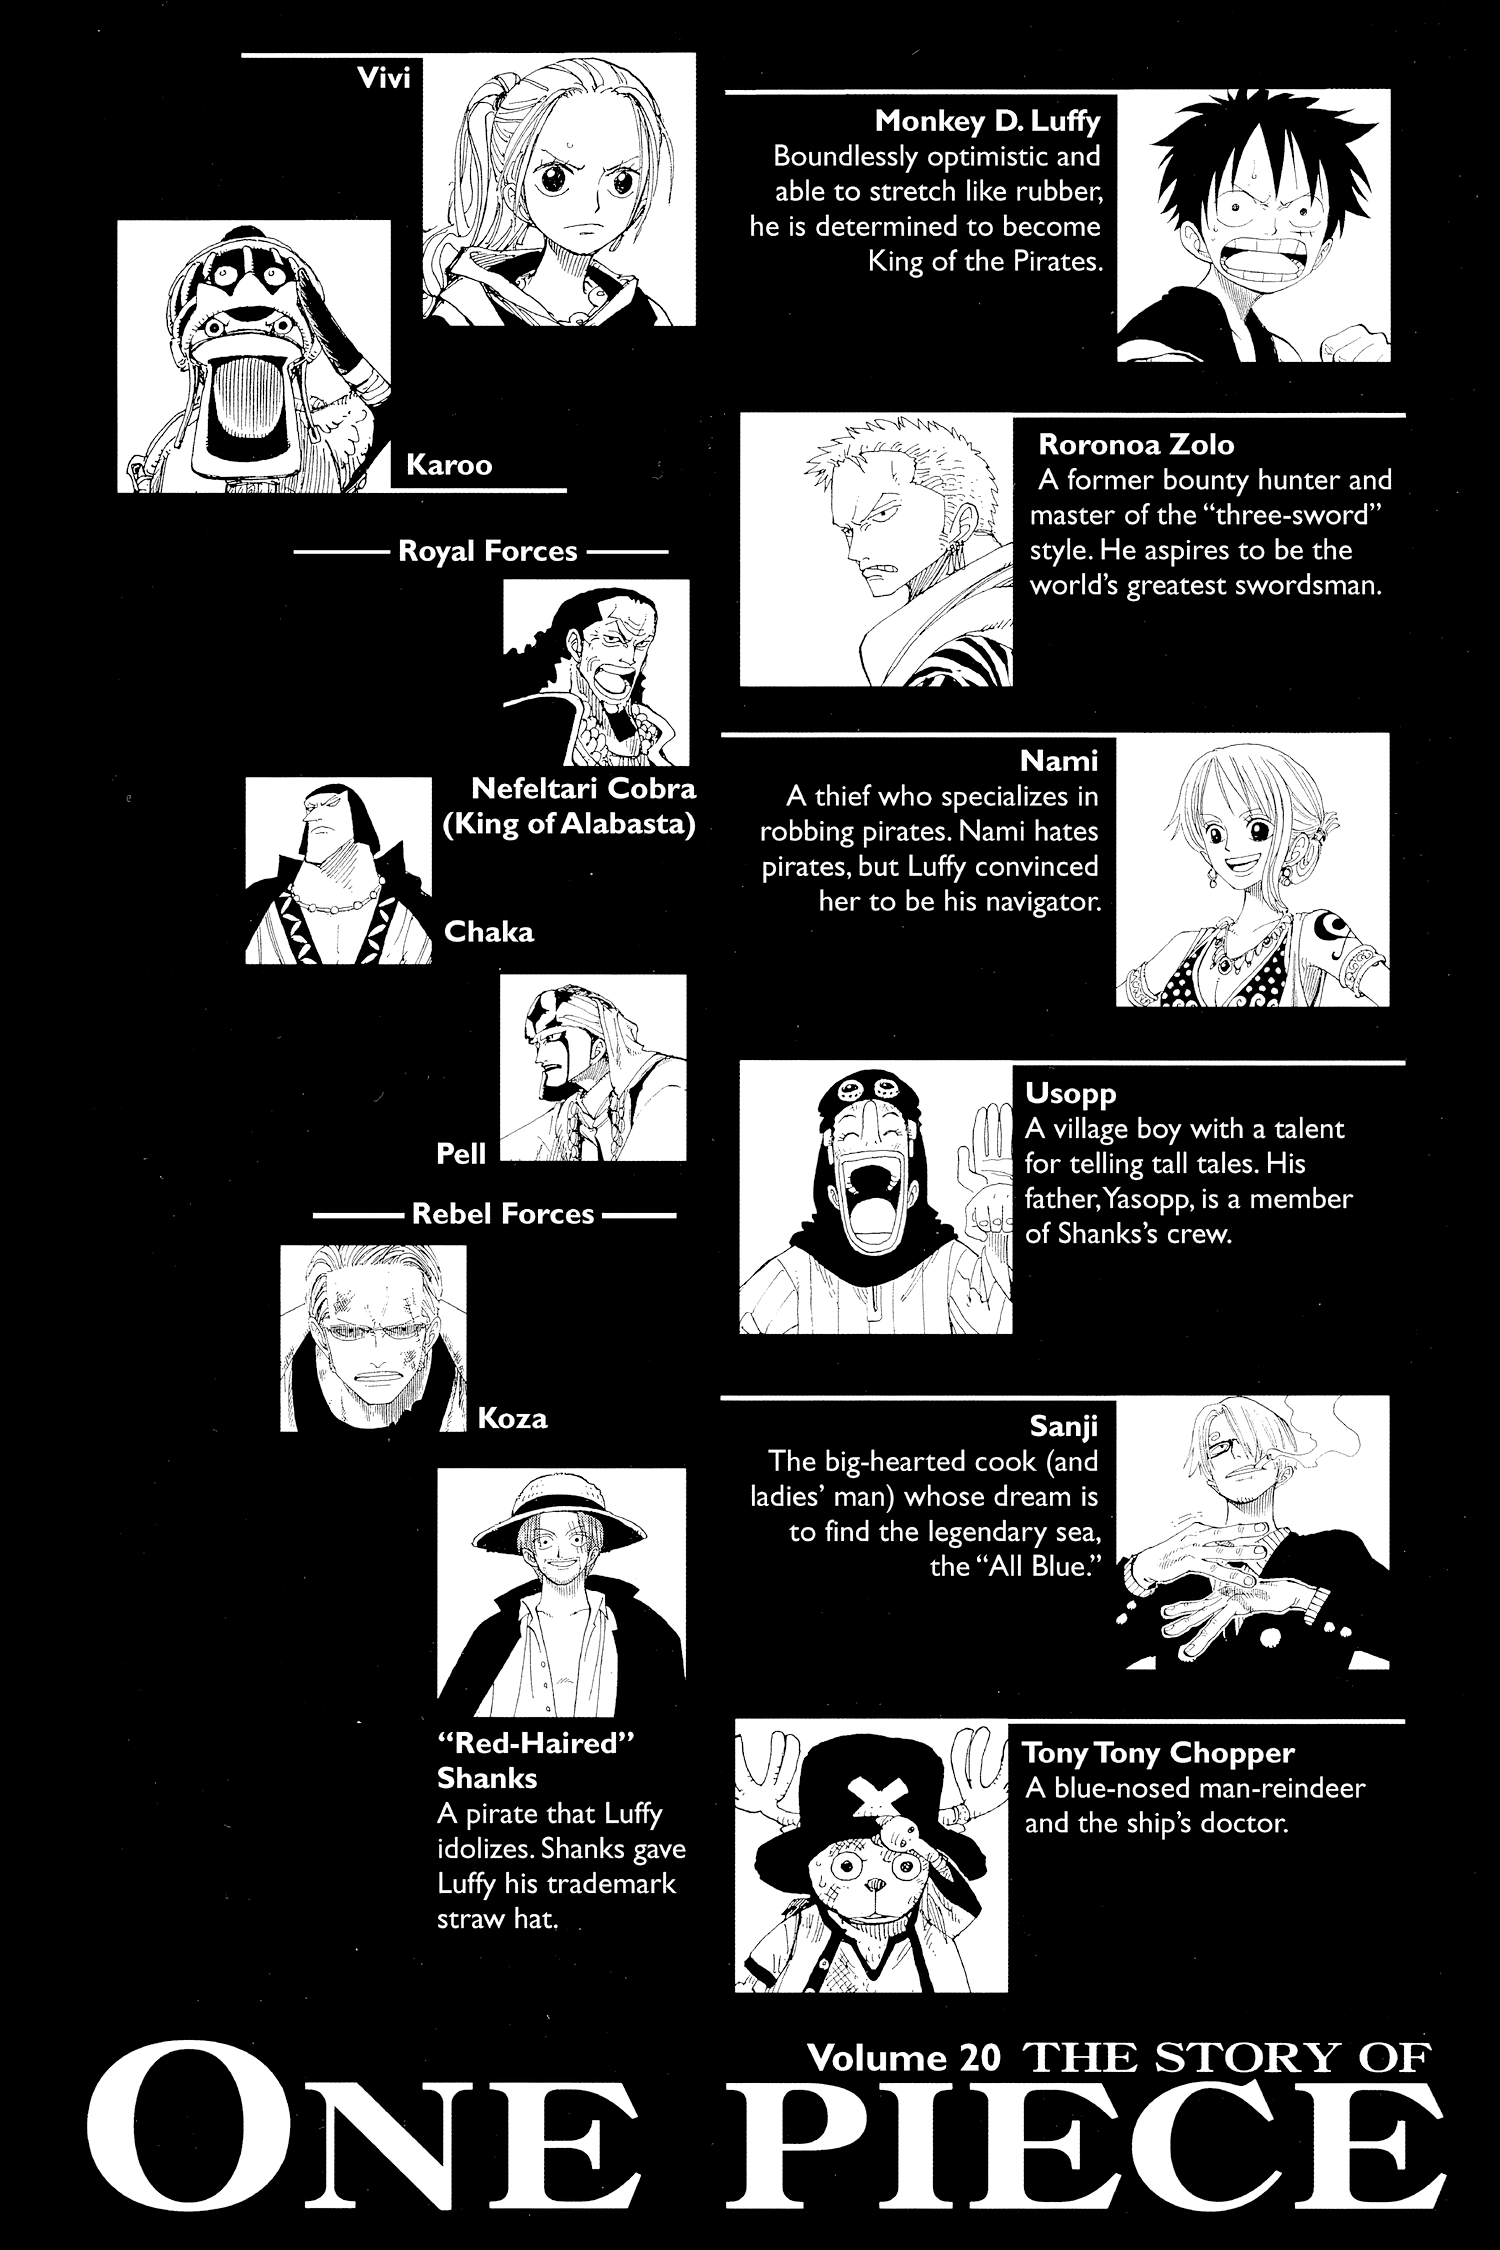
\includegraphics[width=\textwidth]{chapter/output/bad57.png}
      
    \end{subfigure}
    \hfill
    \begin{subfigure}[b]{0.25\textwidth}
        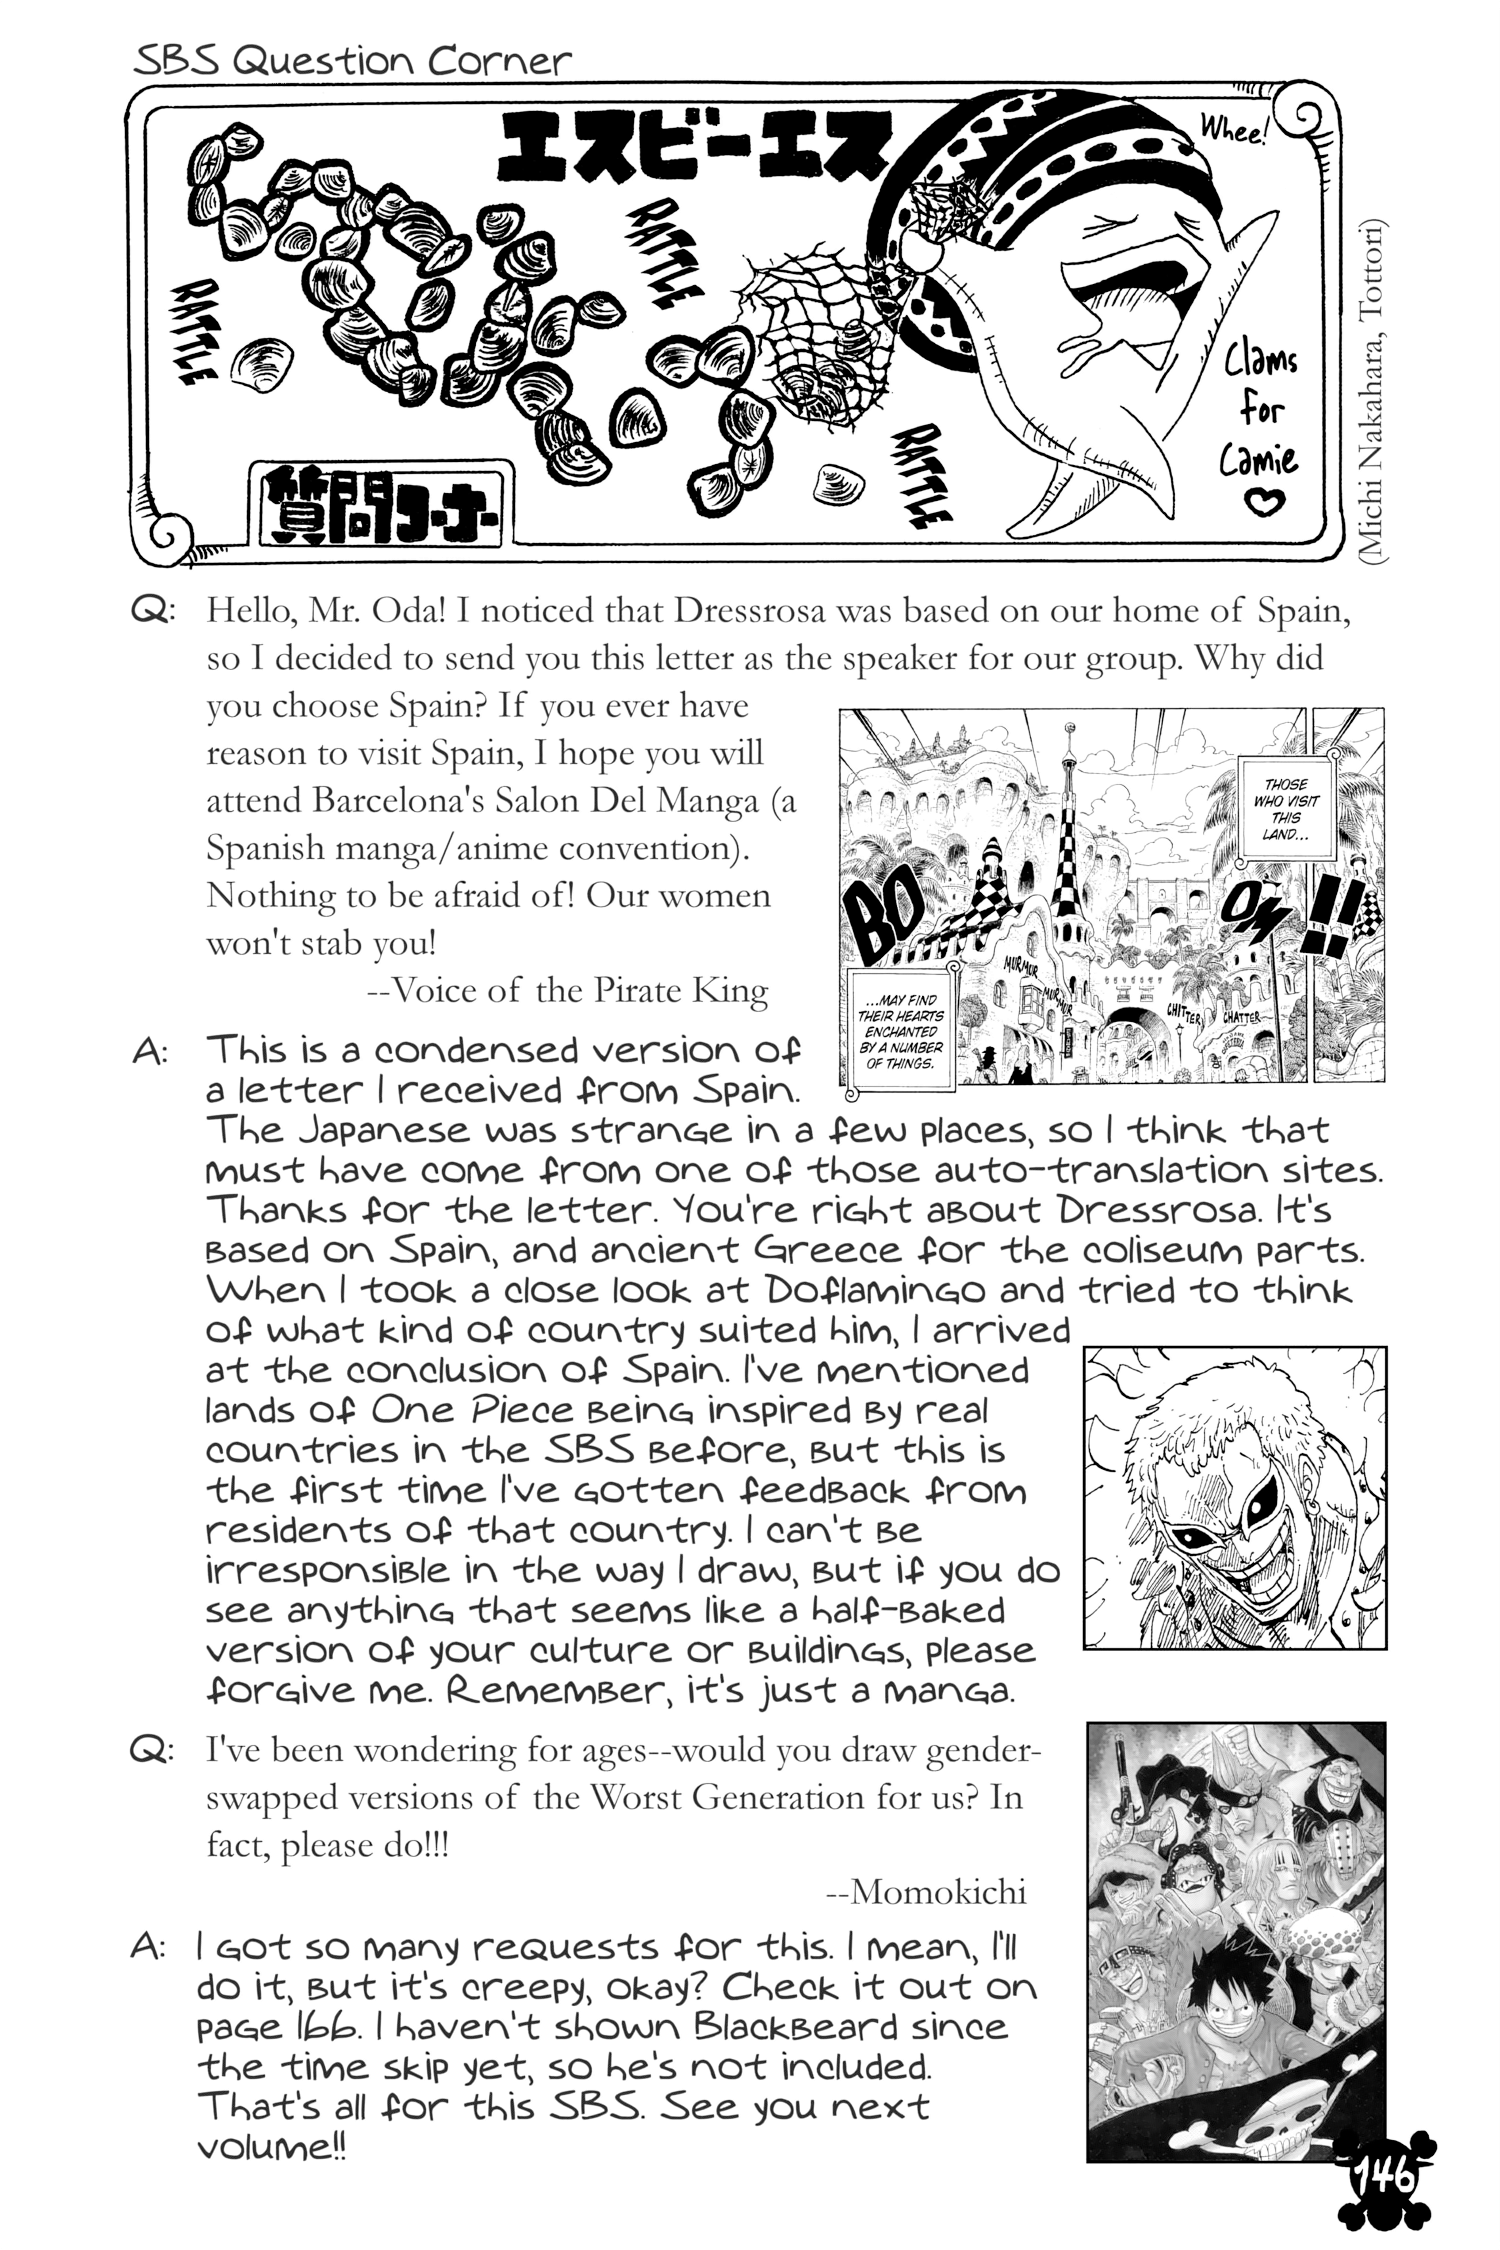
\includegraphics[width=\textwidth]{chapter/output/bw57.png}
        
    \end{subfigure}
    \hfill
    \begin{subfigure}[b]{0.2\textwidth}
        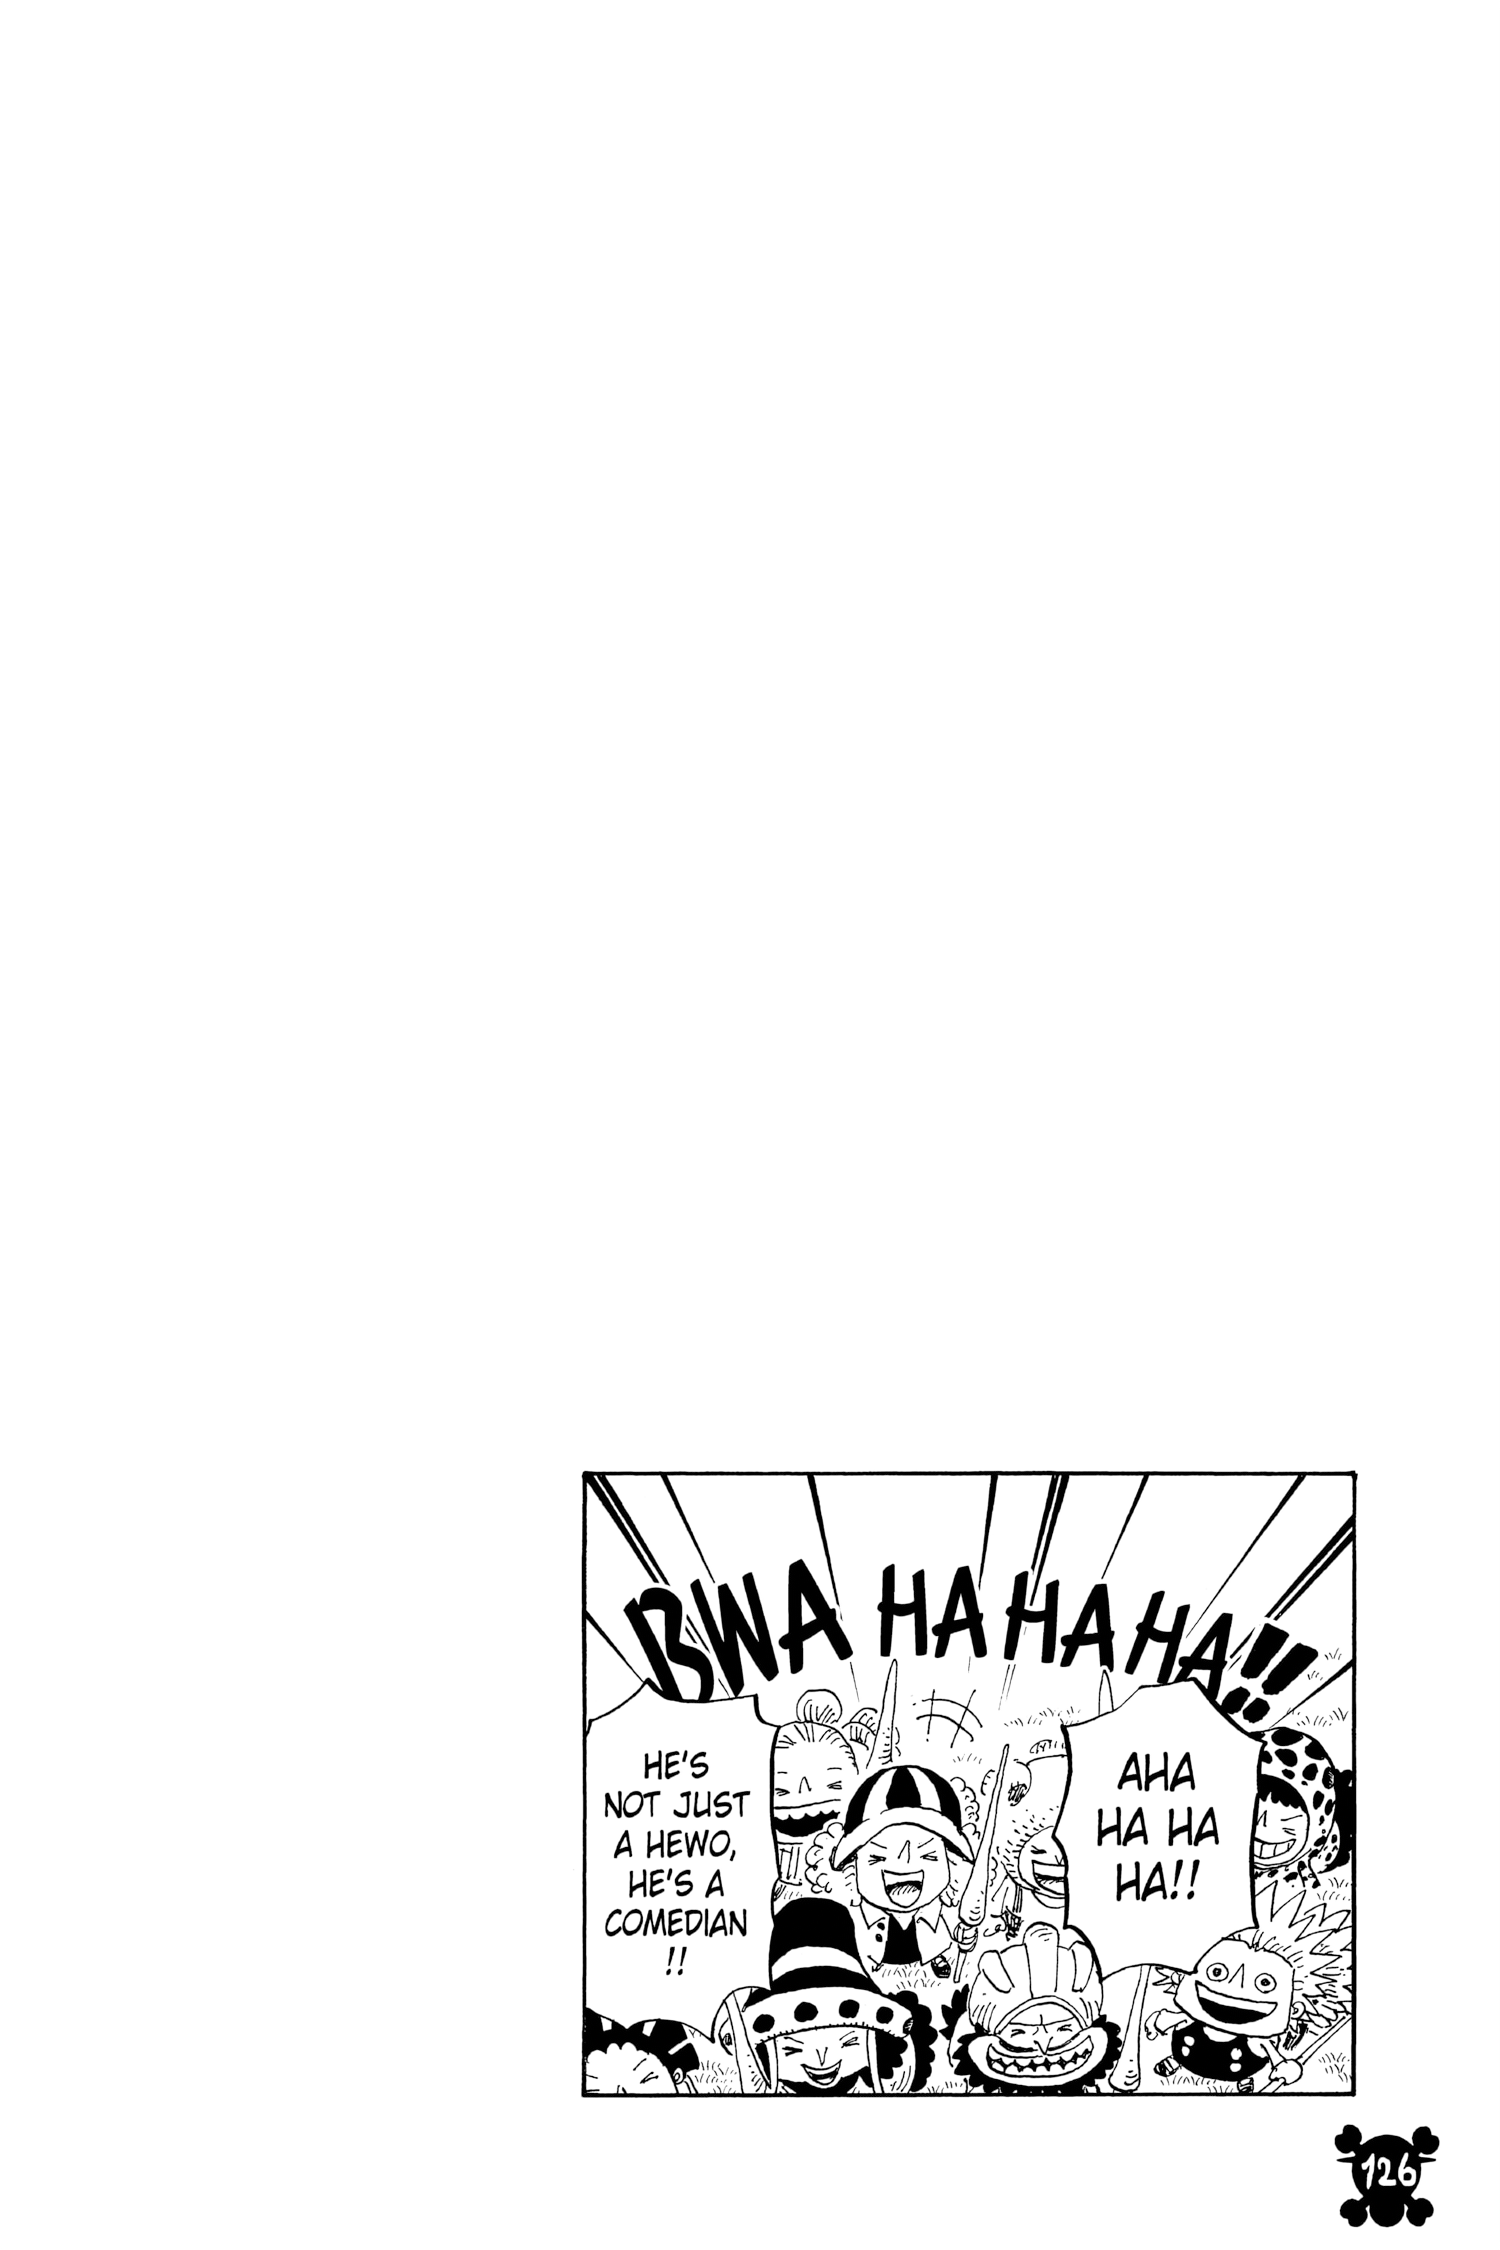
\includegraphics[width=\textwidth]{chapter/output/bw205.png}
       
    \end{subfigure}
    \hfill
    \begin{subfigure}[b]{0.25\textwidth}
        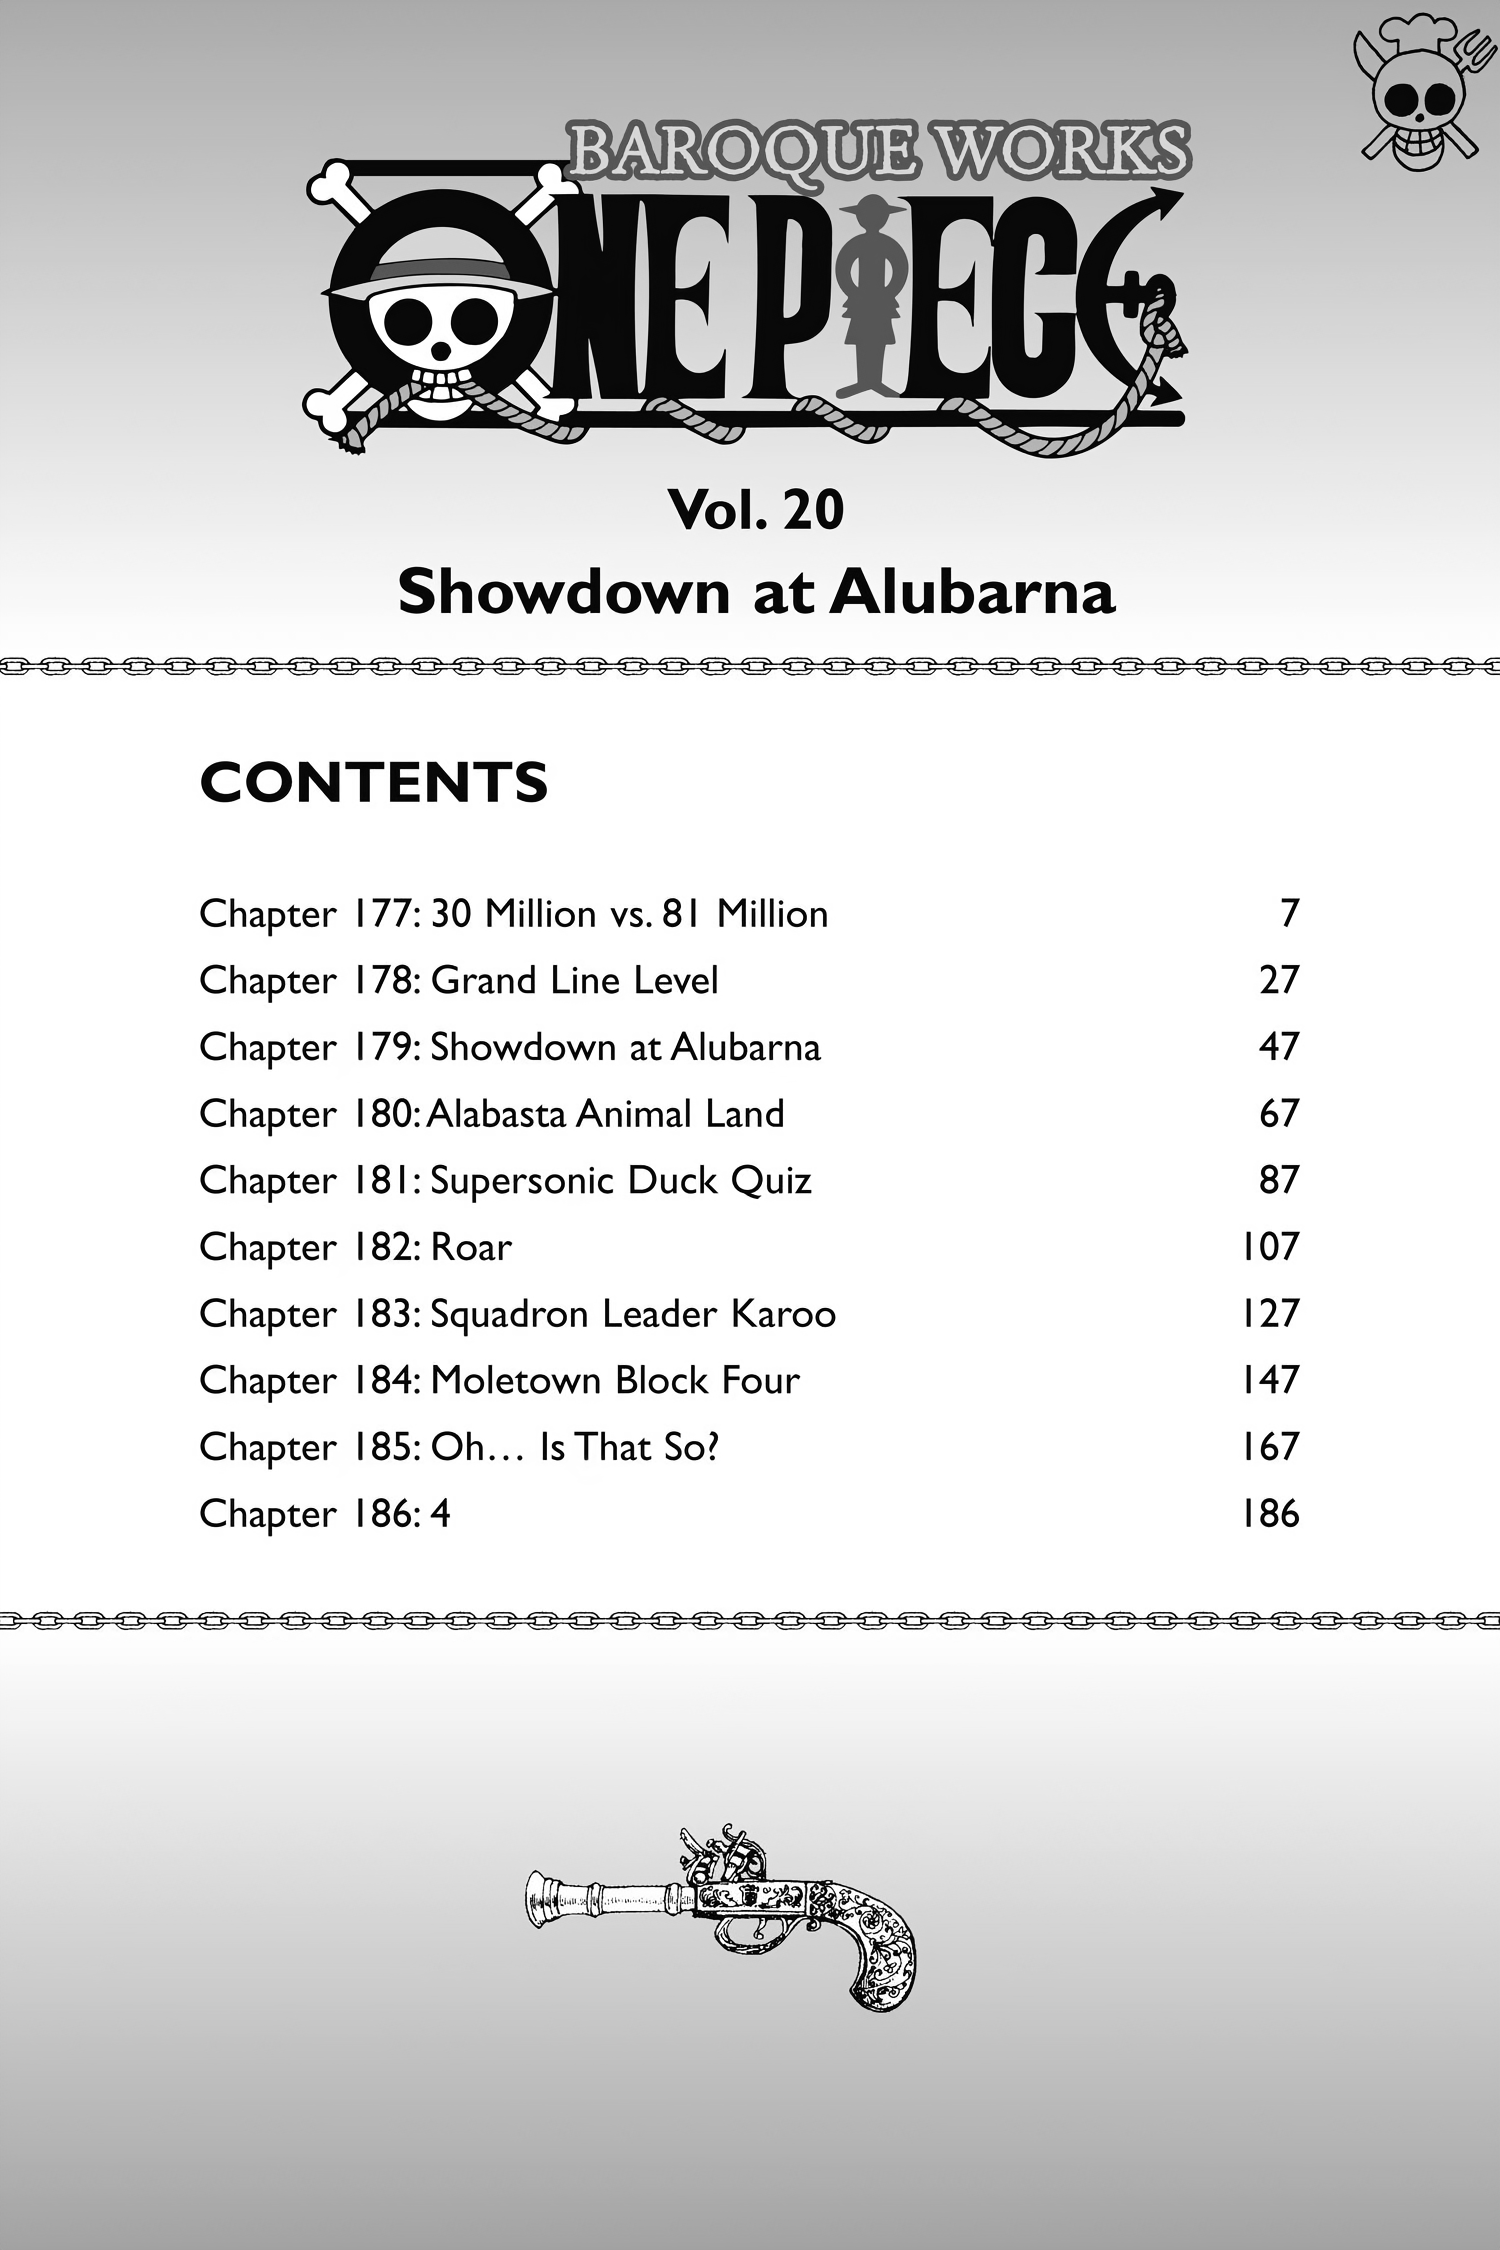
\includegraphics[width=\textwidth]{chapter/output/bad59.png}

    \end{subfigure}
    
    \caption{Bad pages as filtered out by the classifier}
    \label{fig:bad_images}
    
\end{figure}


This refined selection process ensured the model was trained on a focused dataset specifically containing relevant manga artwork. Through these collection and preprocessing steps, we prepared a high-quality, filtered and consistent dataset for our Cycle-GAN model.
\newpage

\section{Model Training}

\subsection{Training a cycle-GAN with UNET Generator}
Initially, we trained a deep UNET with 3 skip connections. The model consisted of multiple Squeeze Extract ResNet. The UNET Model had a total of
32212514 trainable parameters.We used PatchGAN as our discriminator. We trained the model on OnePiece Manga Dataset with Cycle-GAN architecture.
\\
We trained the model for 200 epoch with following parameters:
\begin{itemize}
        \item Learning rate for Color and BW Generators = 1e-4
        \item Learning rate for Color and BW Disciminator = 4e-4
        \item Batch Size = 2
        \item White Color Penalty Threshold = 0.8
        \item Input Image Width = 112
        \item Input Image Height = 112
        \item Model Initialization = Random Initialization
        \item Optimizer = Adam
        \item Adam Optimizer Betas = 0.5, 0.999
        \item Lambda Cycle = 10
\end{itemize}

We evaluated L1 loss, cycle consistency loss and adverserial loss during the training for both
generators and discriminators. Due to its architecture, U-Net Genrator was able to presever the features properly but failed to colorize the image as per our liking. Also, due to the complexity and depth of the generator, we could not accomodate images of size larger than 256x256 in the VRAM. \\
The losses and output during training of the generator is shown below.
\begin{figure}[bp]
    \centering
    \begin{subfigure}[b]{0.45\textwidth}
        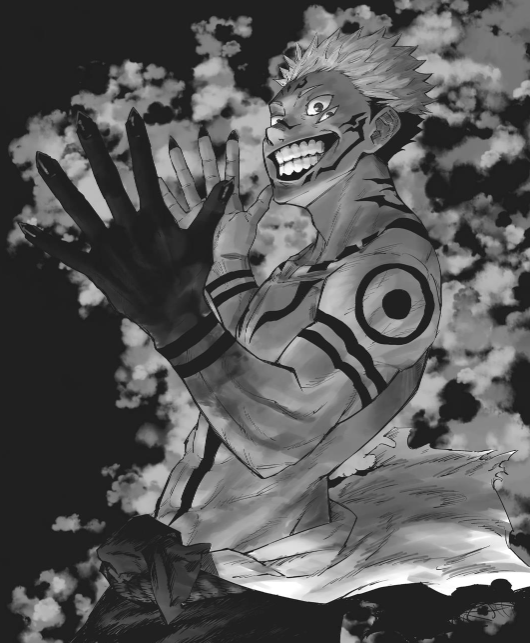
\includegraphics[height=0.8\textwidth]{chapter/output/UNetInput.png}
        \caption{Image Input to UNET}
    \end{subfigure}
    \hfill
    \begin{subfigure}[b]{0.45\textwidth}
        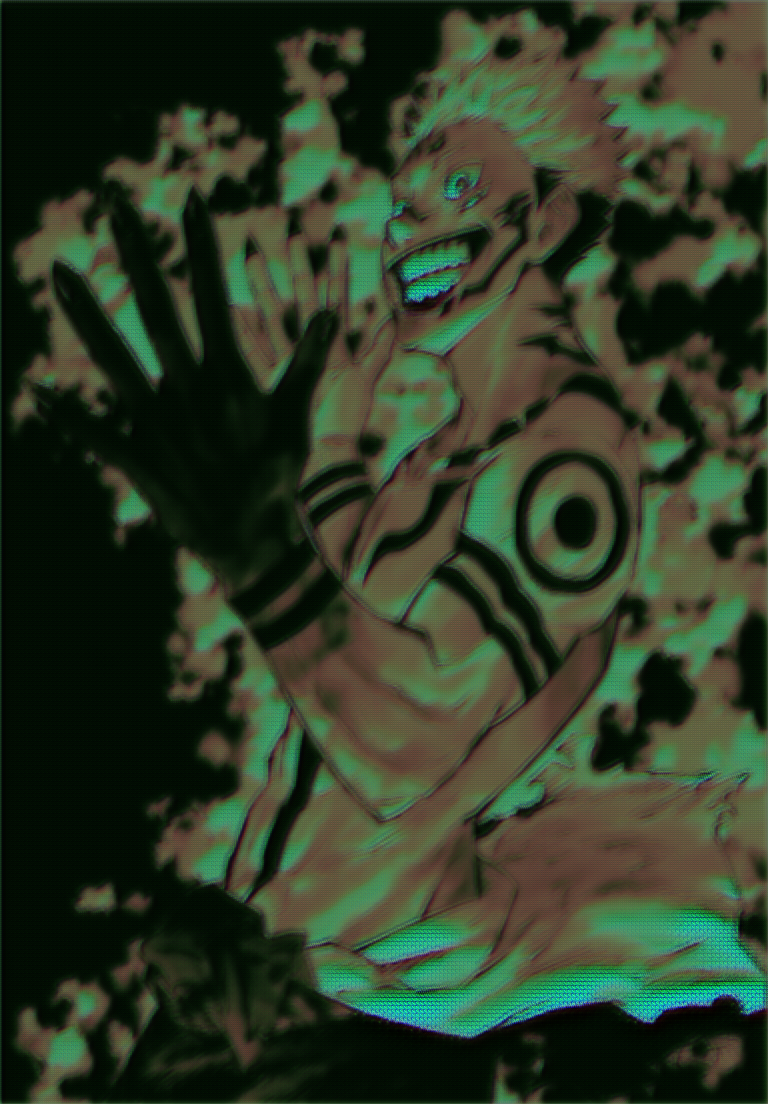
\includegraphics[height=0.8\textwidth]{chapter/output/UNet-output.png}
        \caption{Image Output from UNET}
    \end{subfigure}
    \caption{Output of UNET Generator}
    \label{fig:Output of UNET Generator}
\end{figure}
\newpage

\begin{figure}
    \centering
    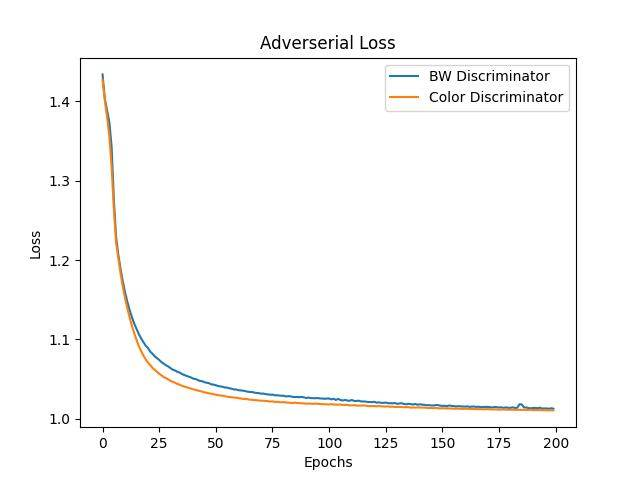
\includegraphics[width=0.7\textwidth]{chapter/output/UNet-adver.jpg}
    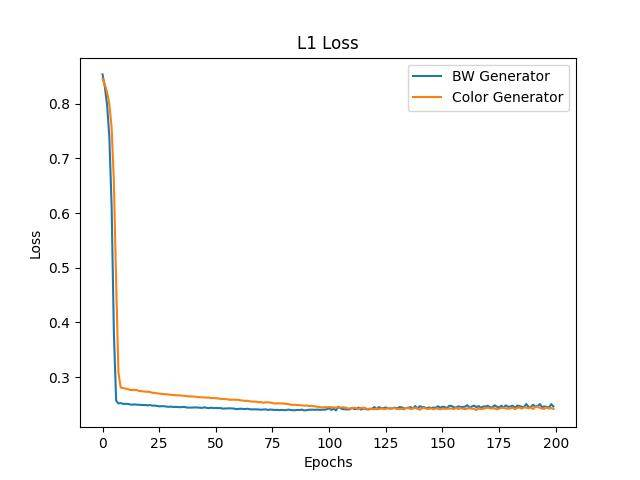
\includegraphics[width=0.7\textwidth]{chapter/output/UNet-l1.jpg}
    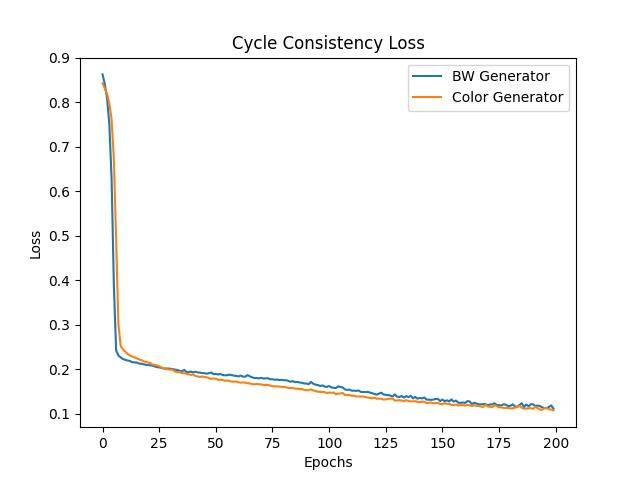
\includegraphics[width=0.7\textwidth]{chapter/output/UNet-cyclecon.jpg}
    \caption{Losses for generators and discriminators.}
    \label{Losses for generators and discriminators.}
\end{figure}
\clearpage


\subsection{Training a Cycle-GAN with Resnet9 Generator}
We realized the simpler ResNet9 generator architecture was able to preserve feature properly (not as much as U-net) and also should be able to colorize as per our liking.
We trained cycleGAN with a ResNet9 generator for both Color, and Black and White Generator. We used a 16x16 PatchGAN as the discriminator. Due to resource and training time constraints, we trained the model with 362 images in both domains from OnePiece Manga Dataset for 200 epochs.
\\
Initially, the images were resized without preserving the aspect ratio of original panel before passing to the model during training. The image outputs at an intermediate training stage have been given in \ref{fig:image_op_train}, which shows the loss of structural information due to resizing. Consequently, when using the so-trained model for inference, it was able to properly color resized images in the order of 256x256 and failed to appropriately fill larger images in original size or aspect ratio. 

So, the model was trained on unresized and cropped images with following parameters.
\begin{itemize}
    \item Number of Epoch = 200
    \item Batch Size = 1
    \item Learning Rate for Generator = 0.0002
    \item Learning Rate for Discriminator = 0.0002
    \item Input Image Width = 256
    \item Input Image Height = 256
    \item Model Initialization = Normal Initialization
    \item Initialization Gain = 0.02
    \item Optimizer = Adam
    \item Adam Optimizer Betas = 0.5, 0.999
    \item Lambda Cycle = 10
    \item Normalization = Instance Normalization
\end{itemize}
\newpage
\begin{figure}
    \centering
      \begin{subfigure}[b]{0.3\textwidth}
        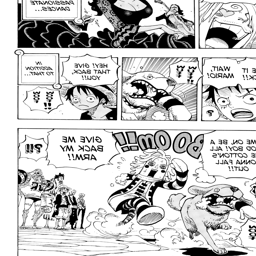
\includegraphics[width=\textwidth]{chapter/output/epoch100_real_A.png}
        \caption{Real BW}
    \end{subfigure}  
    \hfill
    \begin{subfigure}[b]{0.3\textwidth}
        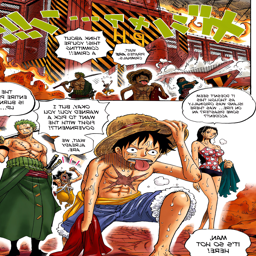
\includegraphics[width=\textwidth]{chapter/output/epoch100_real_B.png}
        \caption{Real Color}
    \end{subfigure}
\end{figure}

\begin{figure}
\centering
    \begin{subfigure}[b]{0.3\textwidth}
        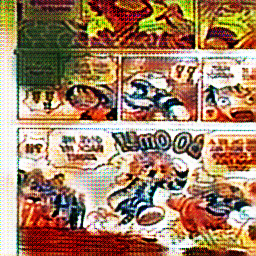
\includegraphics[width=\textwidth]{chapter/output/epoch100_fake_B.png}
        \caption{Fake Color}
    \end{subfigure}
    \hfill
    \begin{subfigure}[b]{0.3\textwidth}
        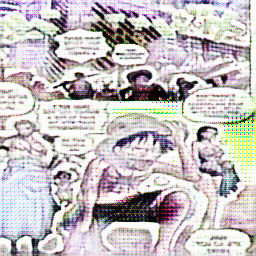
\includegraphics[width=\textwidth]{chapter/output/epoch100_fake_A.png}
        \caption{Fake BW}
    \end{subfigure}

\end{figure}

\begin{figure}
    \centering

    \begin{subfigure}[b]{0.3\textwidth}
        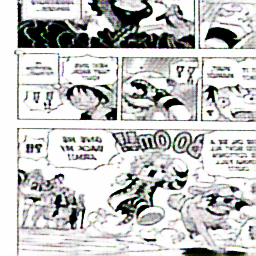
\includegraphics[width=\textwidth]{chapter/output/epoch100_idt_B.png}
       \caption{Identity BW}
    \end{subfigure}
    \hfill
    \begin{subfigure}[b]{0.3\textwidth}
        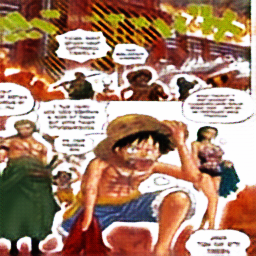
\includegraphics[width=\textwidth]{chapter/output/epoch100_idt_A.png}
        \caption{Identity Color}
    \end{subfigure}

\end{figure}



\begin{figure}  
    \centering
    \begin{subfigure}[b]{0.3\textwidth}
        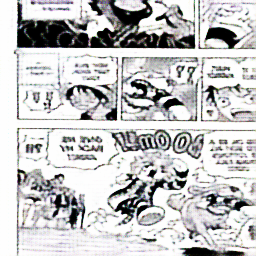
\includegraphics[width=\textwidth]{chapter/output/epoch100_rec_A.png}
        \caption{Recreated BW}
    \end{subfigure}
    \hfill
    \begin{subfigure}[b]{0.3\textwidth}
        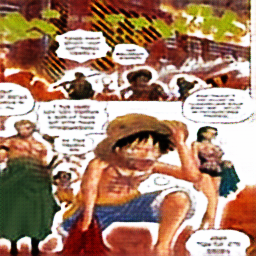
\includegraphics[width=\textwidth]{chapter/output/epoch100_rec_B.png}
        \caption{Recreated Color}
    \end{subfigure}
    
    \caption{Images output during training}
    \label{fig:bad_images}
    
\end{figure}

%---------------------------------gen flowchart
\begin{figure}[hbtp]
  \centering
  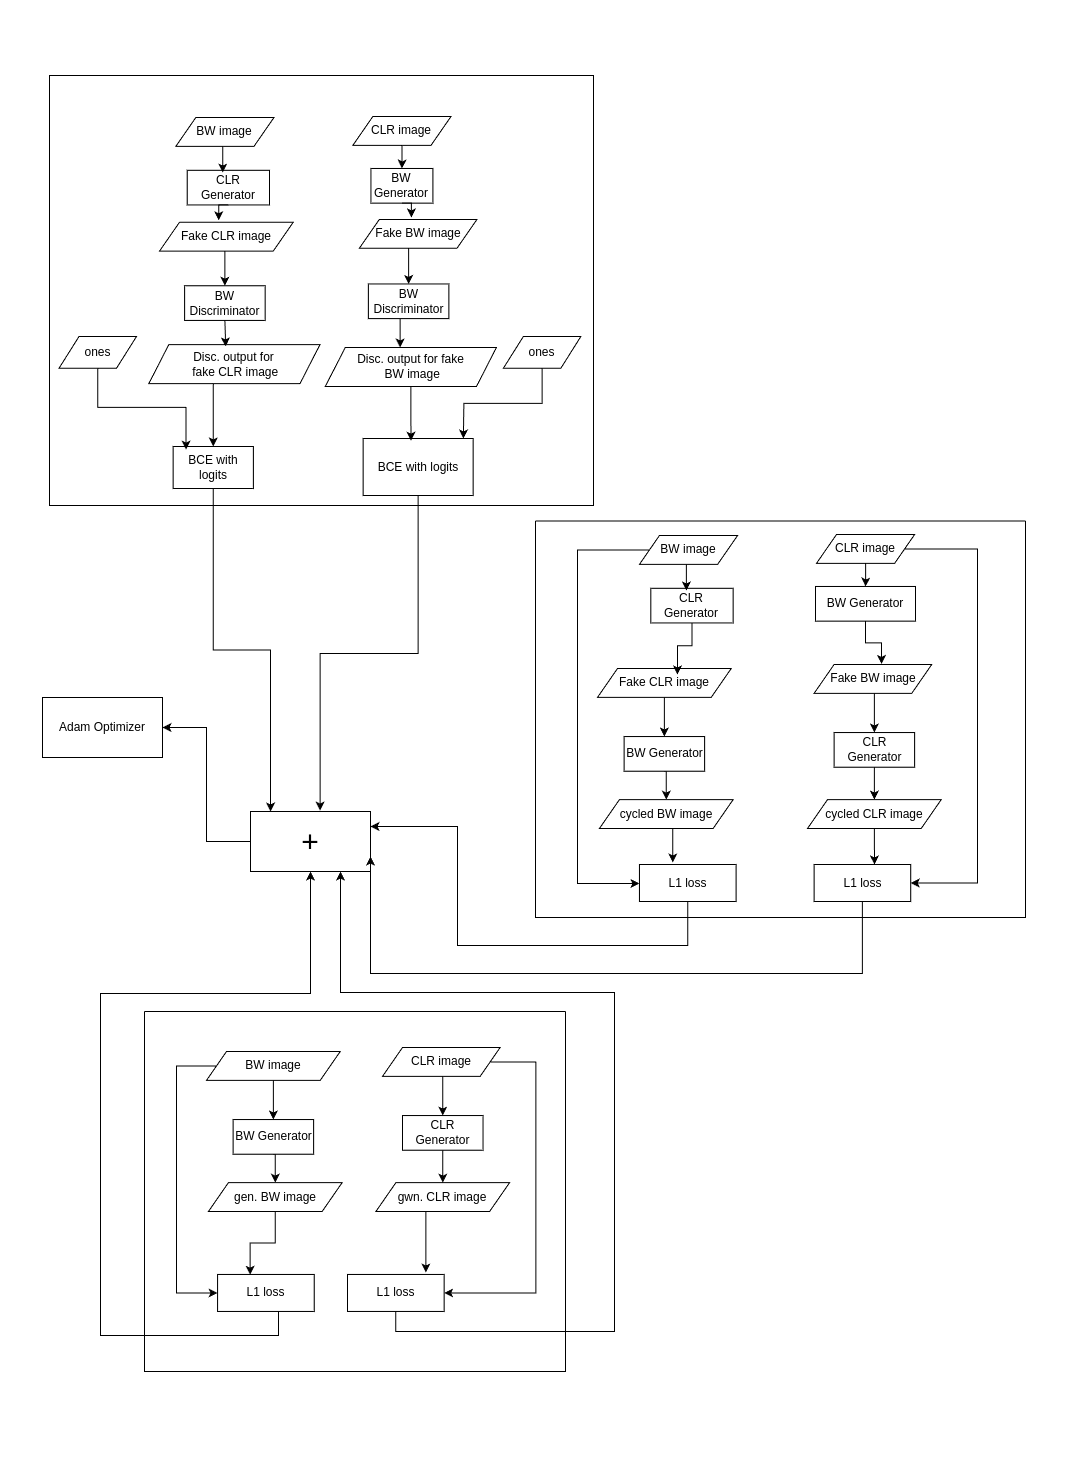
\includegraphics[width=1.1\textwidth]{chapter/img_procedure/generator_procedure_full.png}
  \caption{Generator Training Procedure }
  \label{Generator Training Procedure}
\end{figure}
%--------------------------------- disc flowchart

\begin{figure}[hbtp]
  \centering
  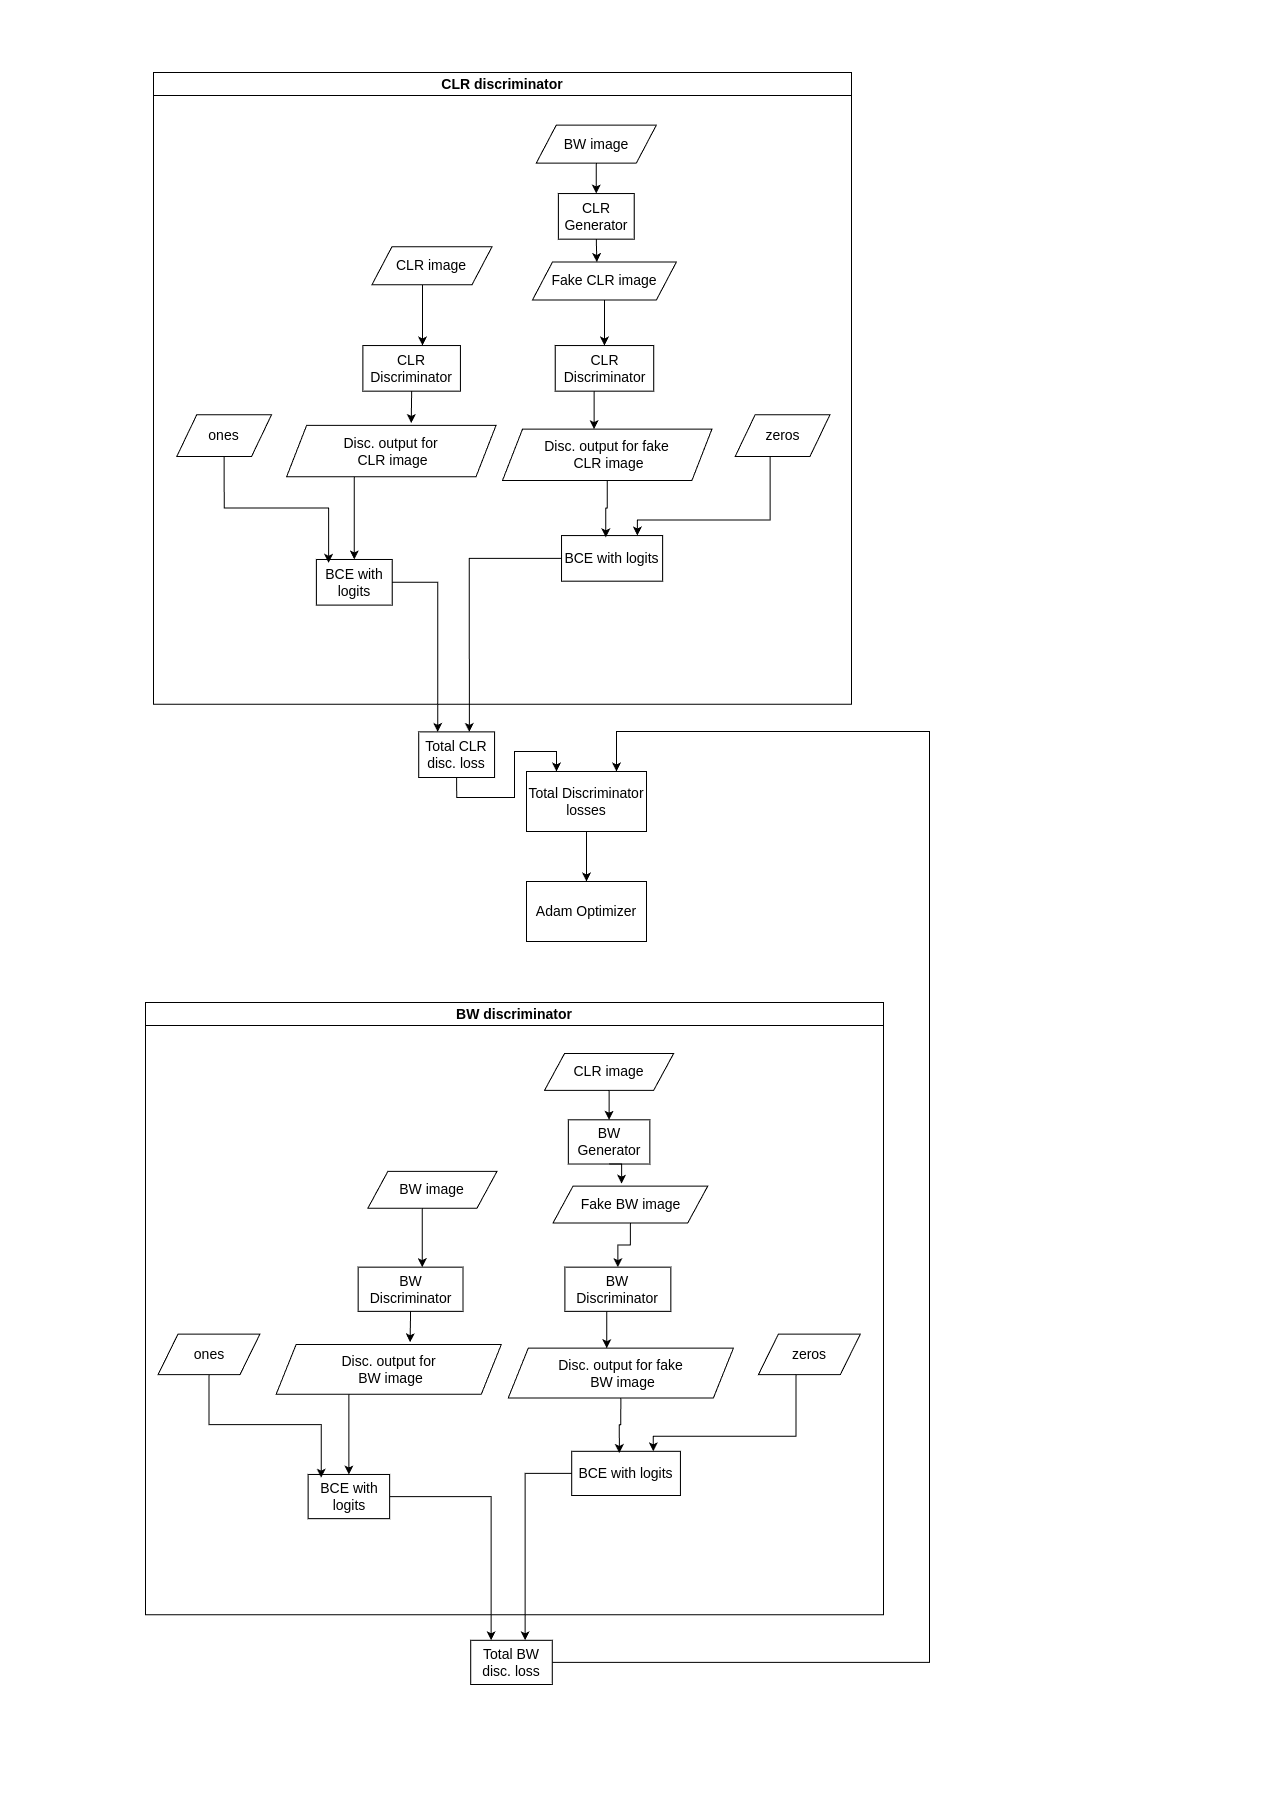
\includegraphics[width=1.2\textwidth]{chapter/img_procedure/disc_procedure_full.png}
  \caption{Discriminator Training Procedure }
  \label{Discriminator Training Procedure}
\end{figure}
%-----------------------------------------------------

\begin{figure}[htbp]
    \centering
    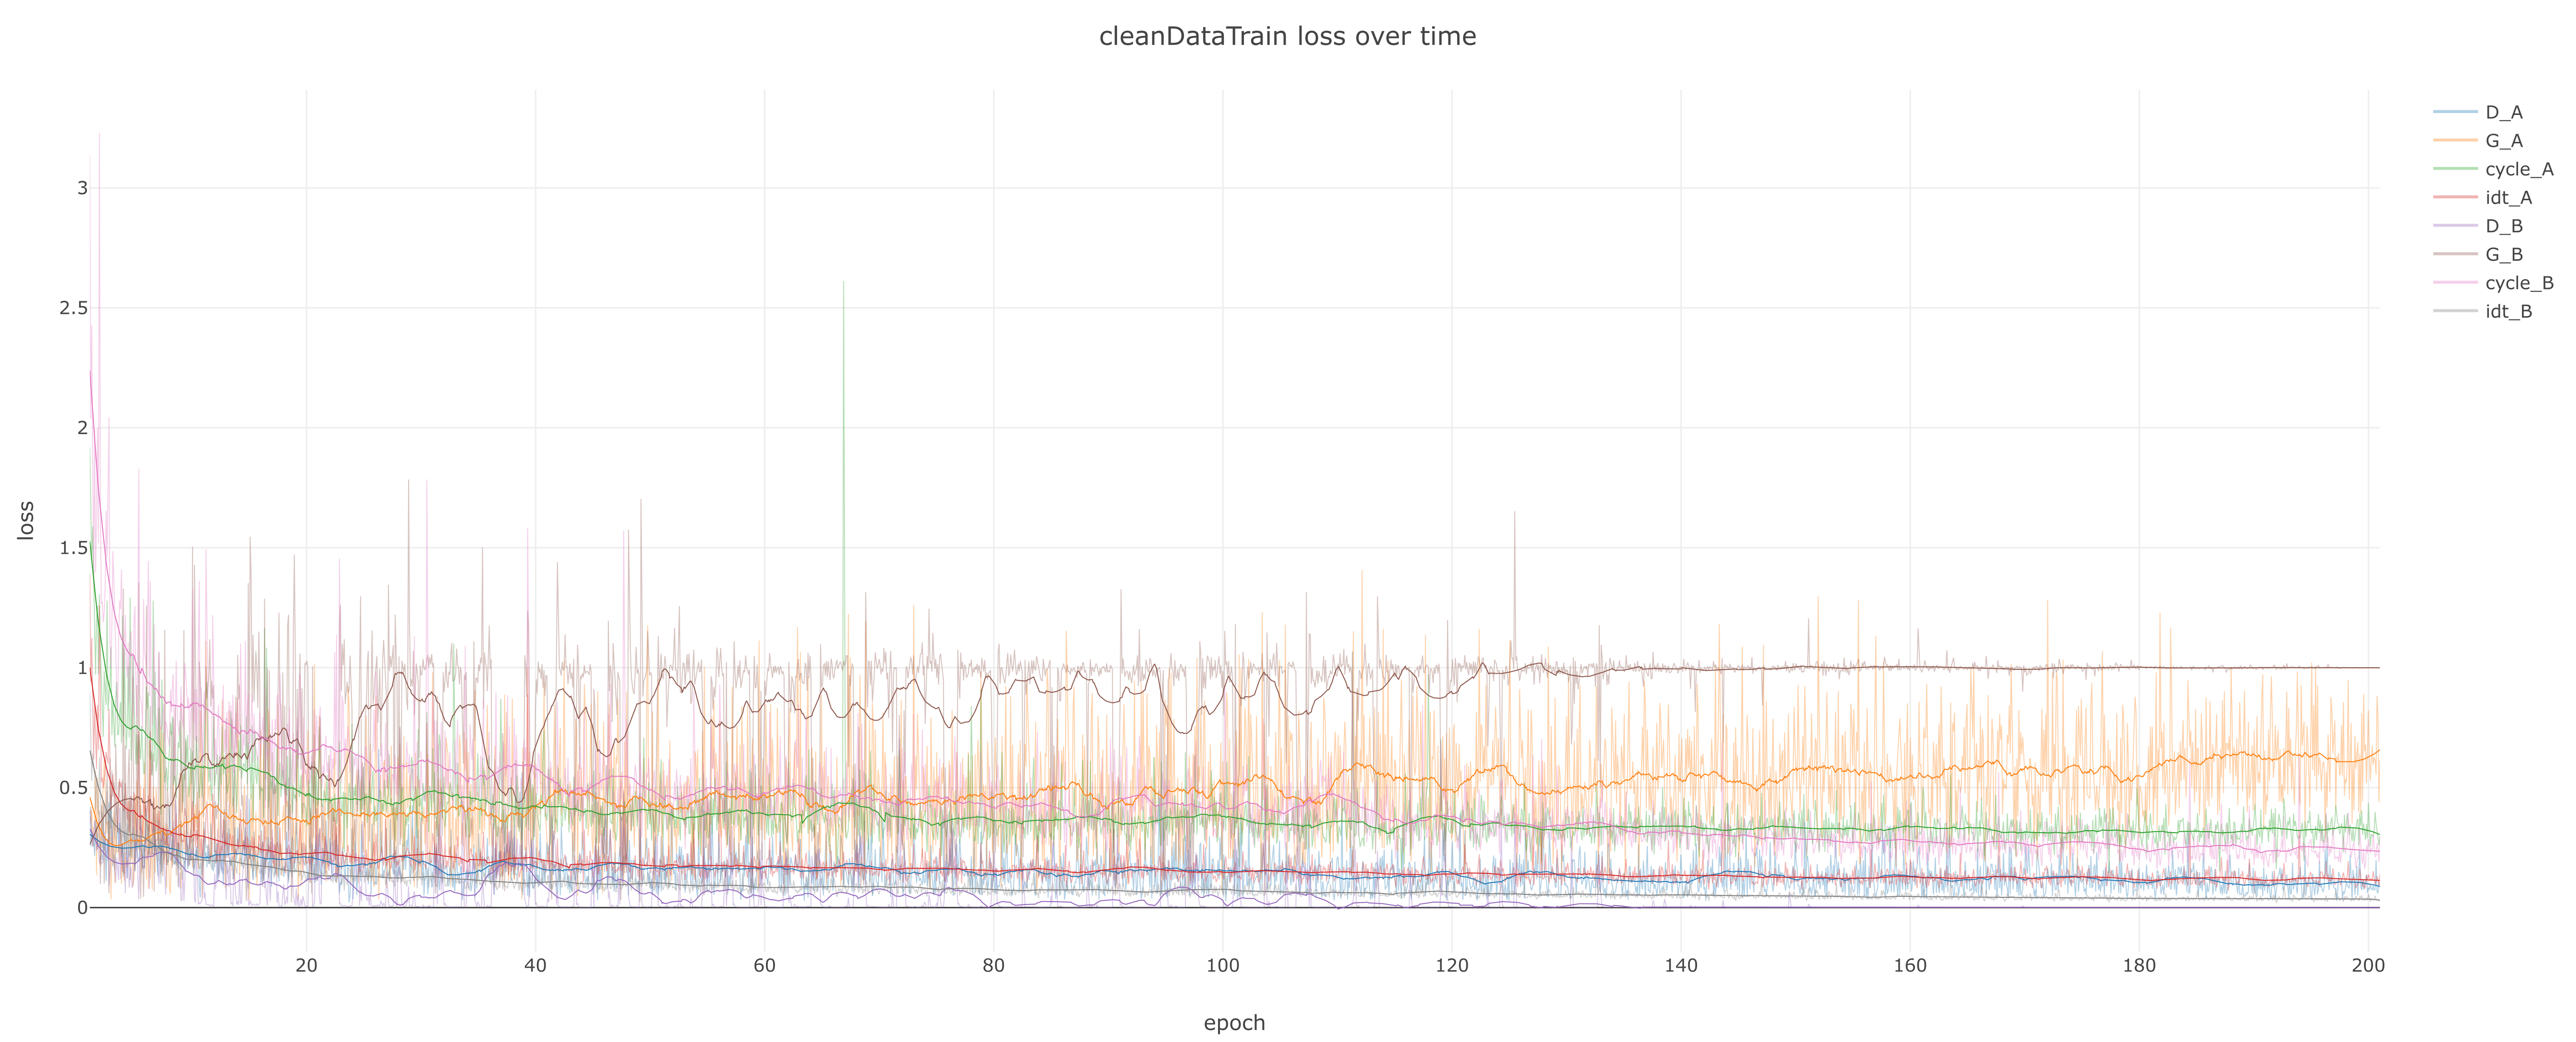
\includegraphics[width=1\textwidth]{chapter/losses_png/all.png}
    \caption{Losses for training with ResNet9Generator and PatchGAN}

    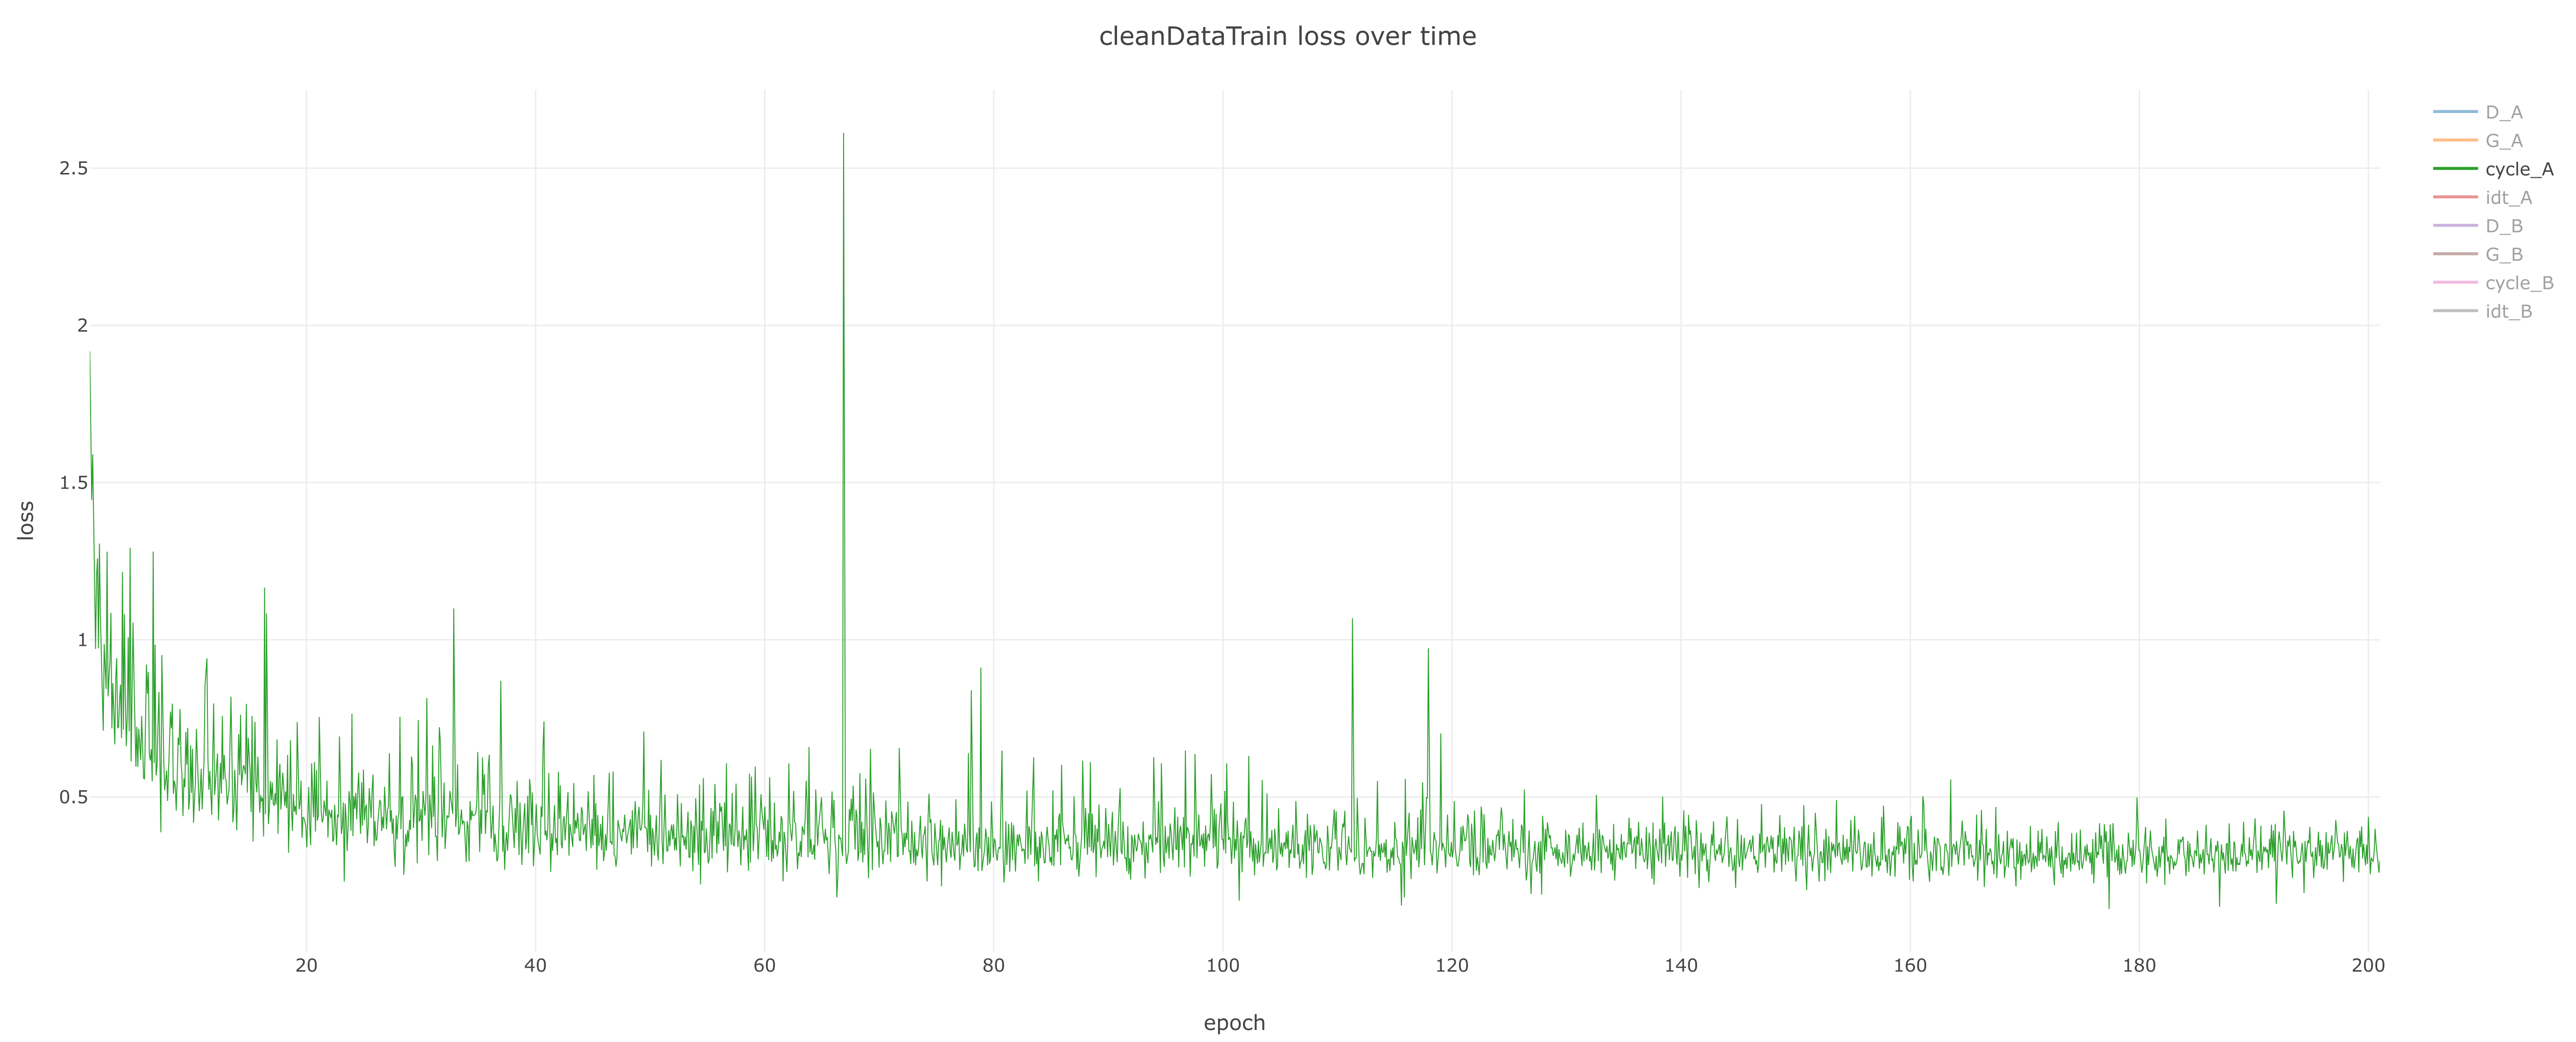
\includegraphics[width=1\textwidth]{chapter/losses_png/cycle_a.png}
    \caption{Cycle Consistency Loss (L1) for Color Generator}
    
    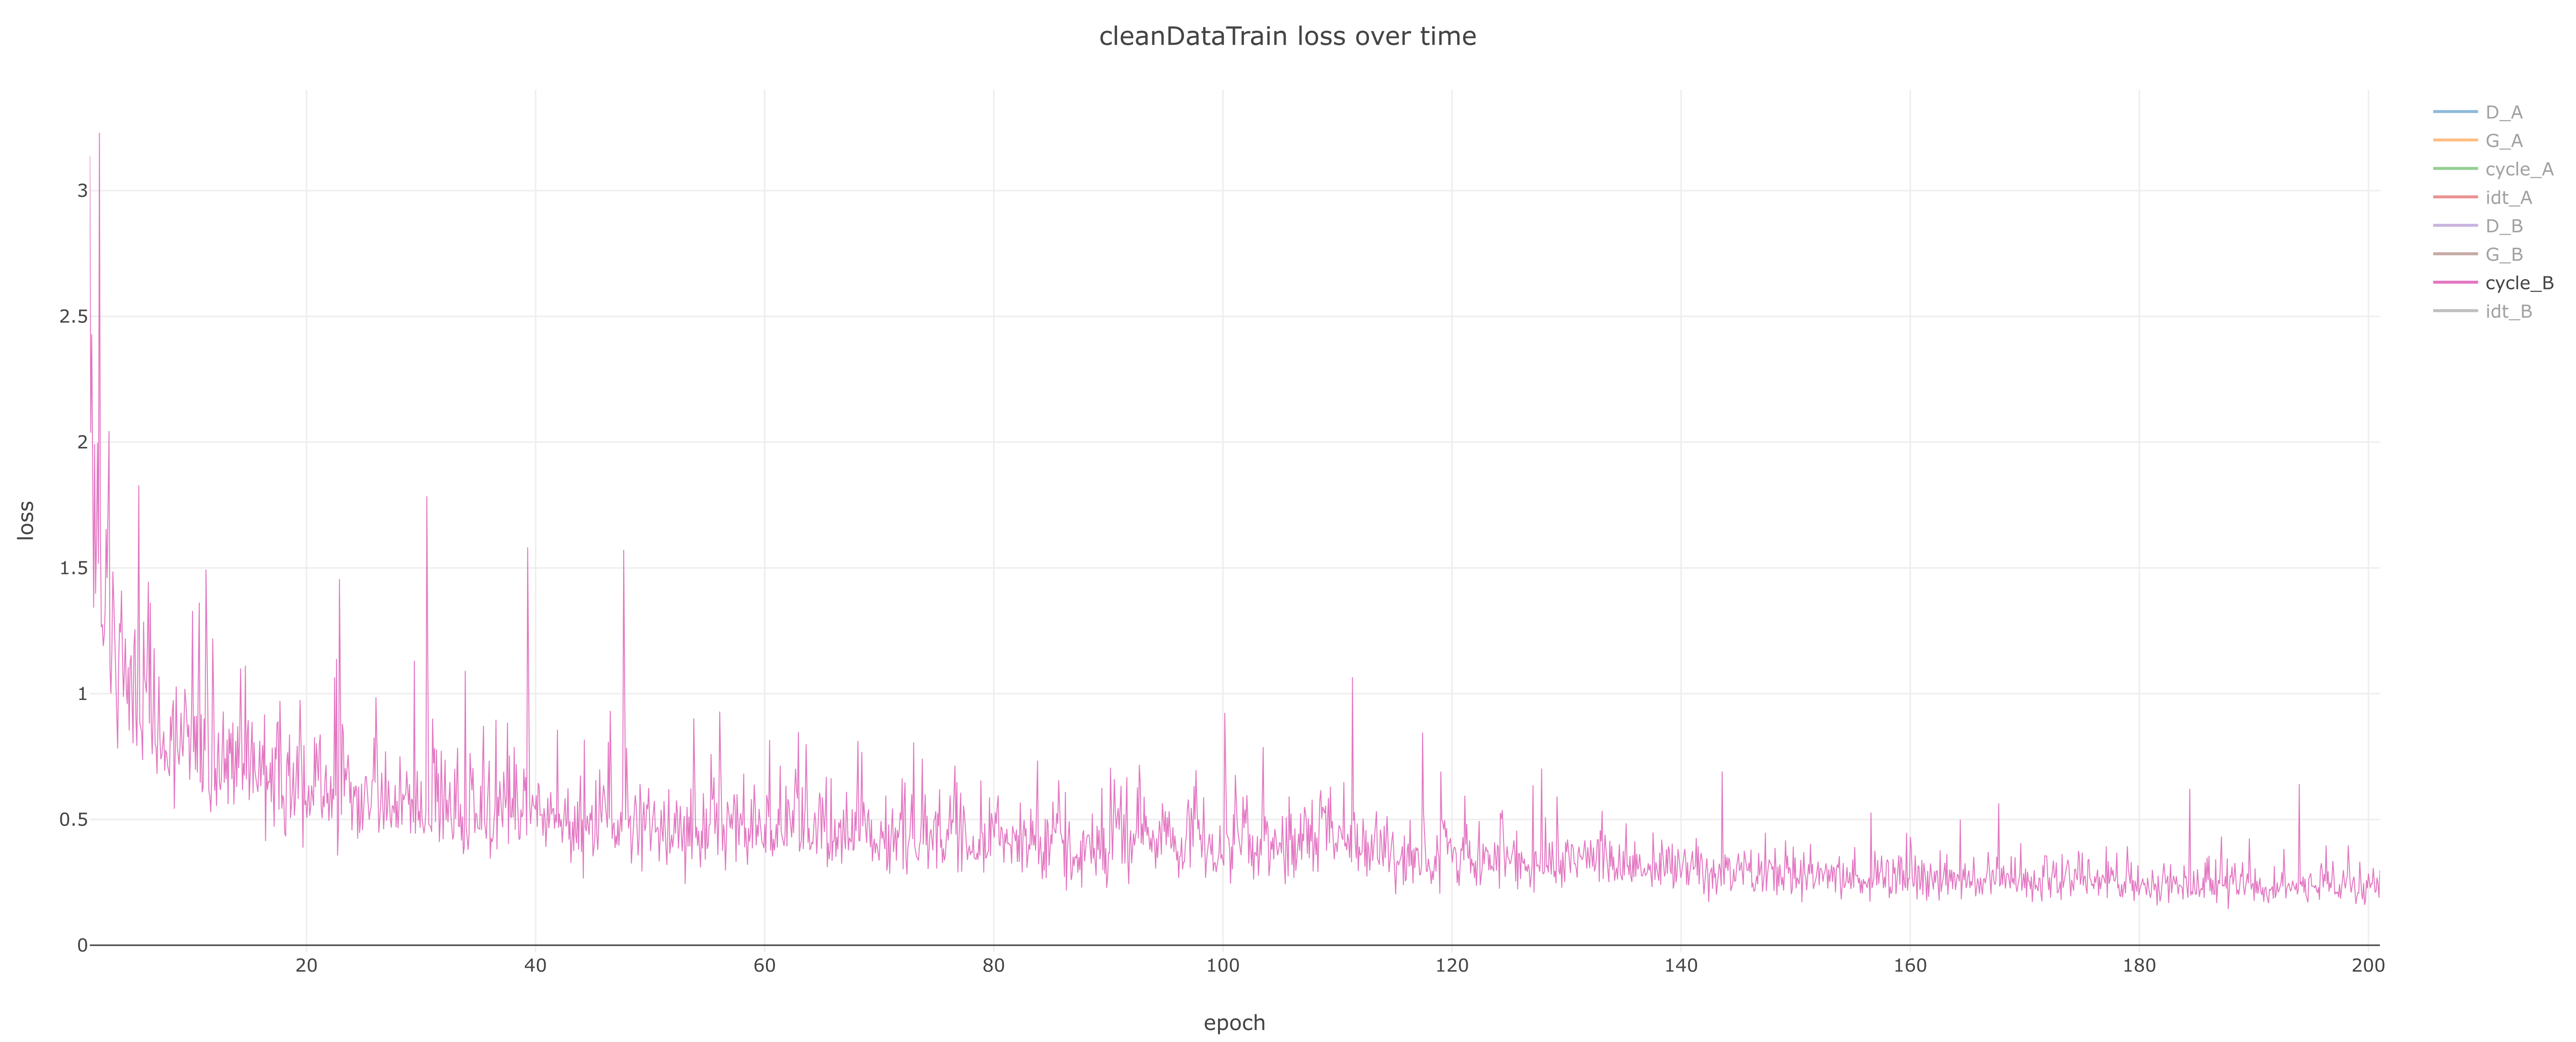
\includegraphics[width=1\textwidth]{chapter/losses_png/cycle_b.png}
    \caption{Cycle Consistency Loss (L1) for BW Generator}
    \end{figure}
    \pagebreak
    \newpage
    \begin{figure}[htbp]
    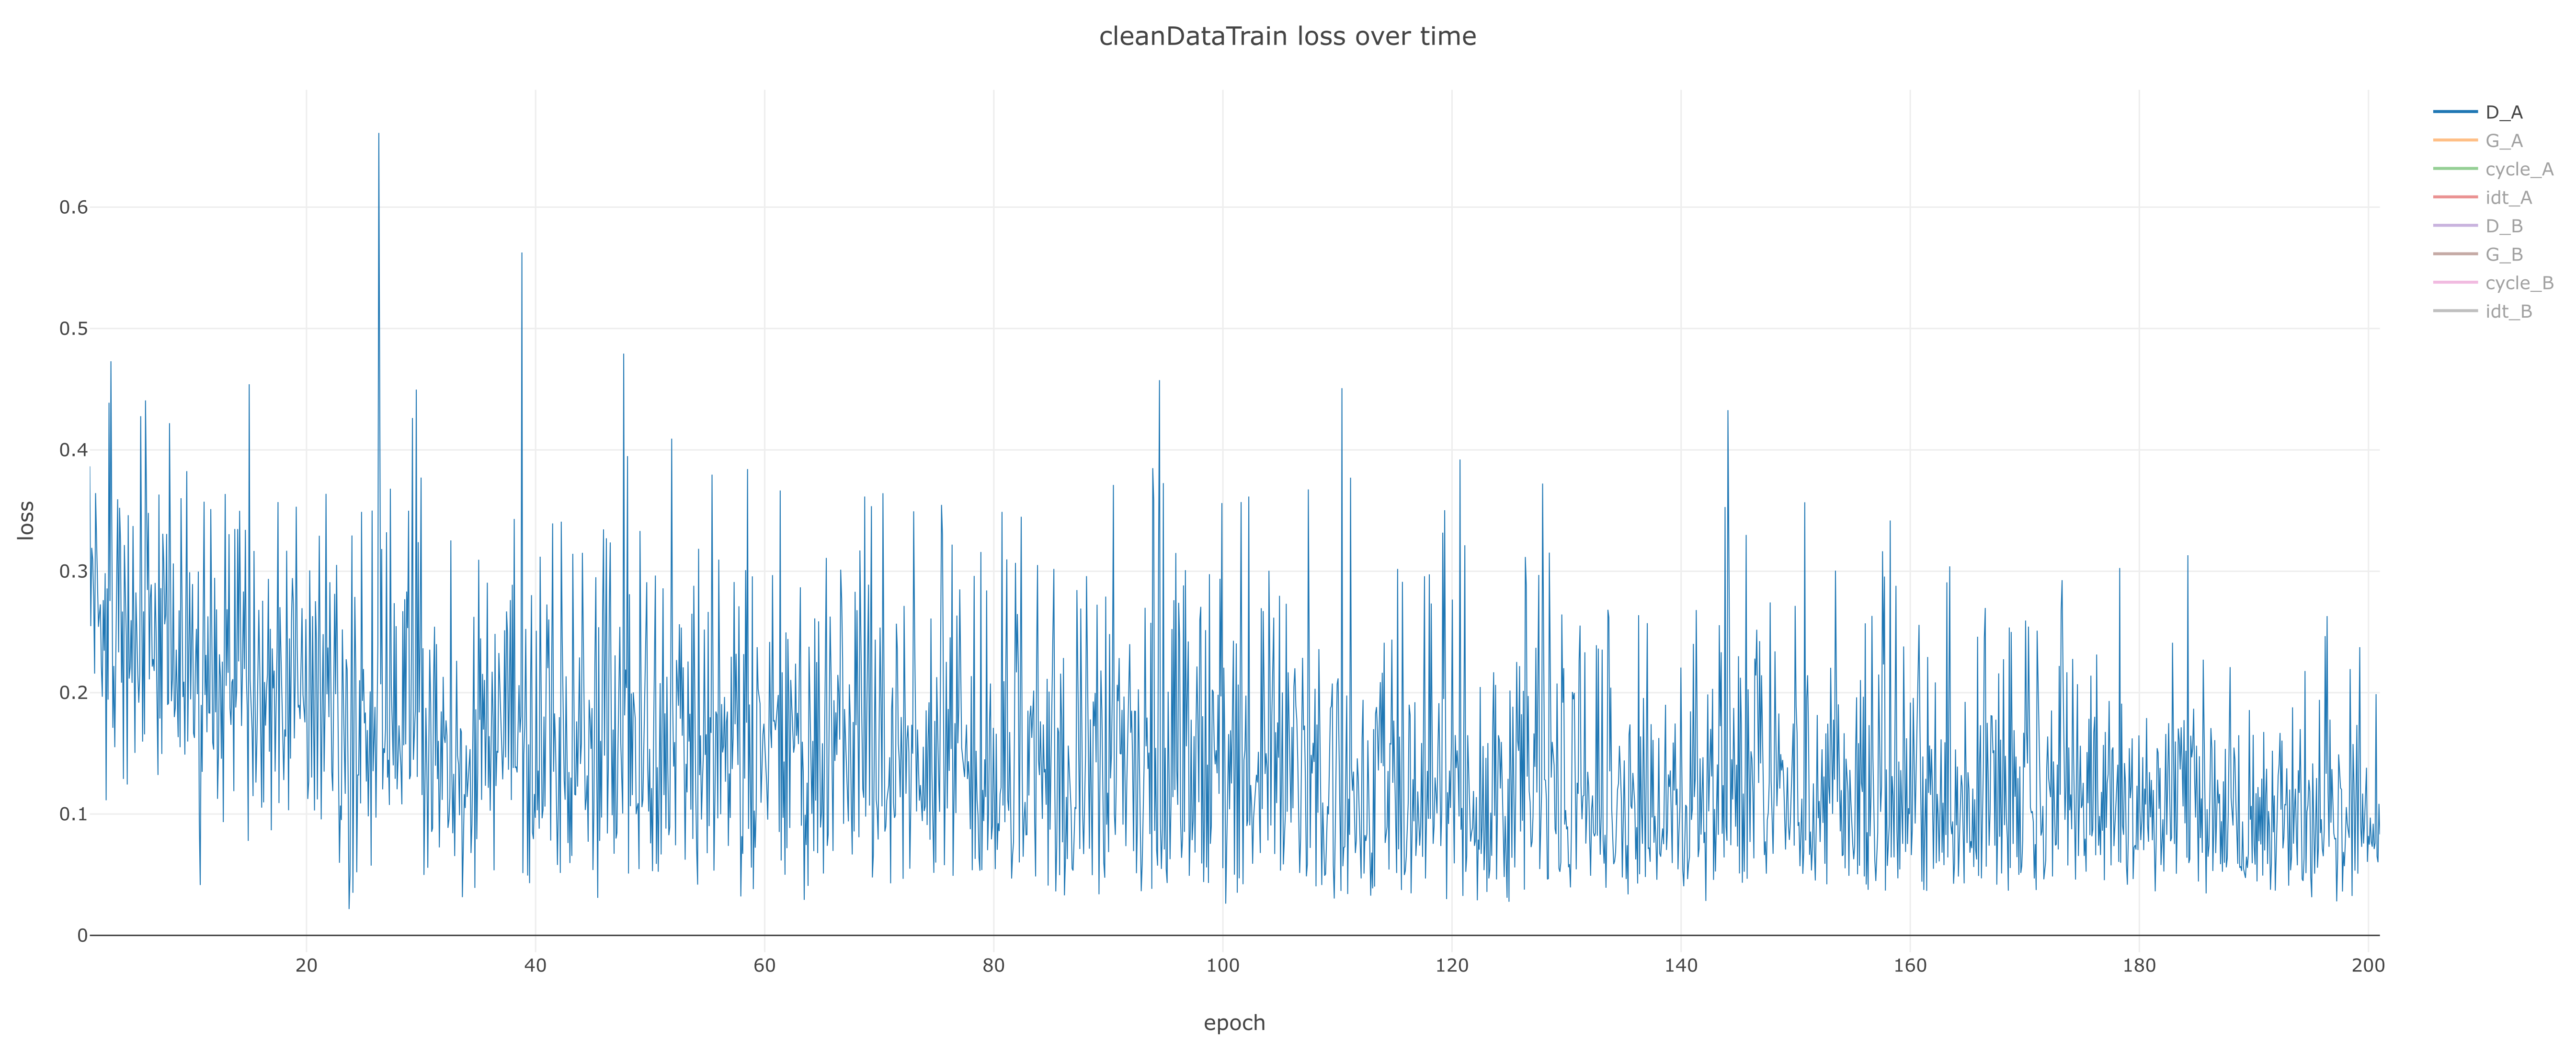
\includegraphics[width=1\textwidth]{chapter/losses_png/d_a.png}
    \caption{BCE Loss for Color Discriminator}
    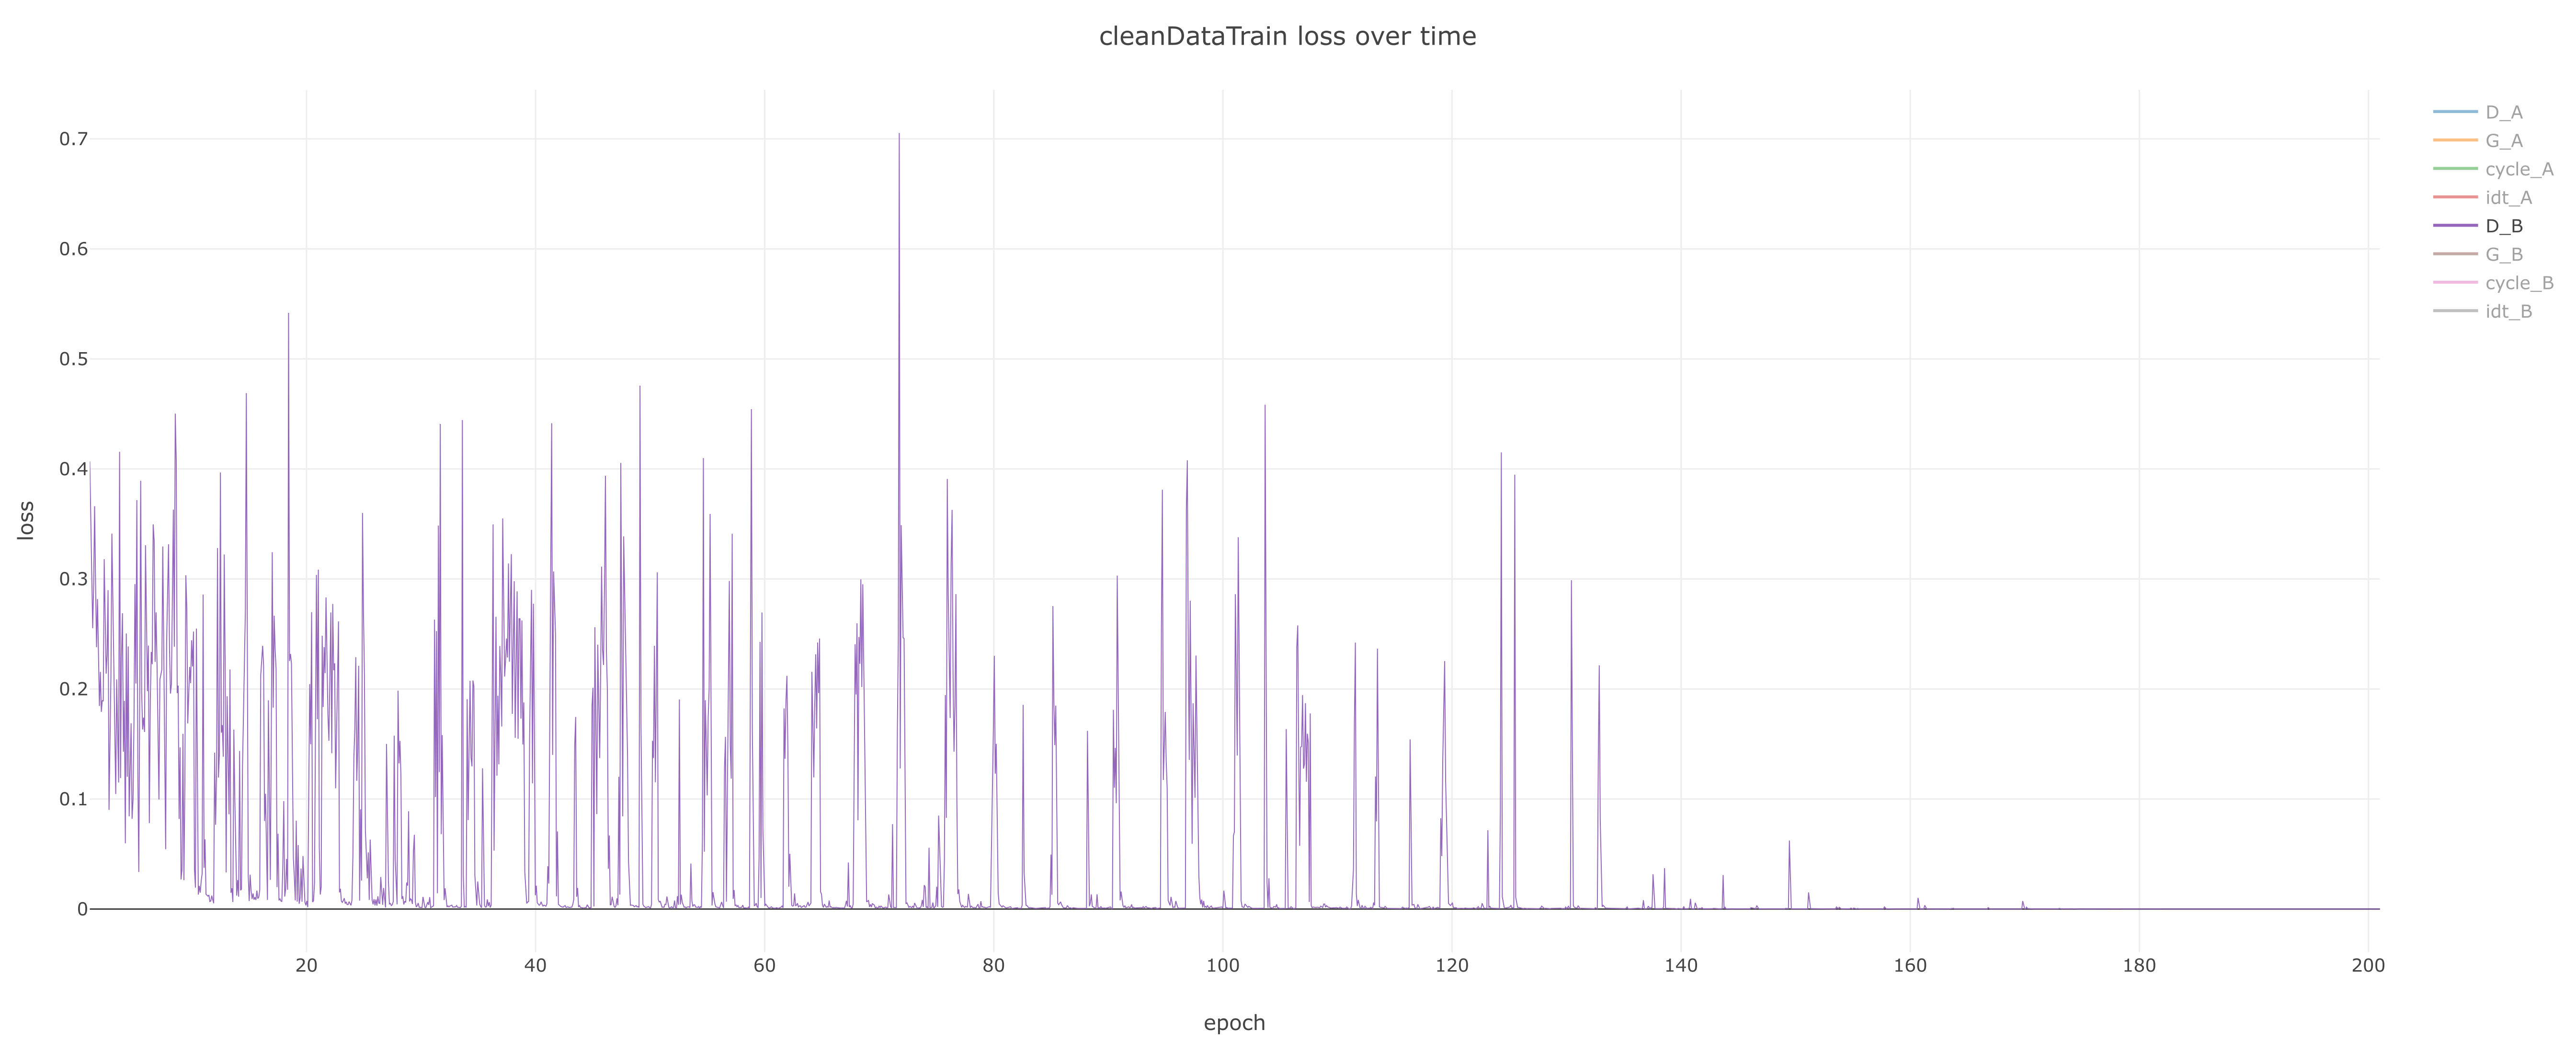
\includegraphics[width=1\textwidth]{chapter/losses_png/d_b.png}
    \caption{BCE Loss for BW Discriminator}
    
    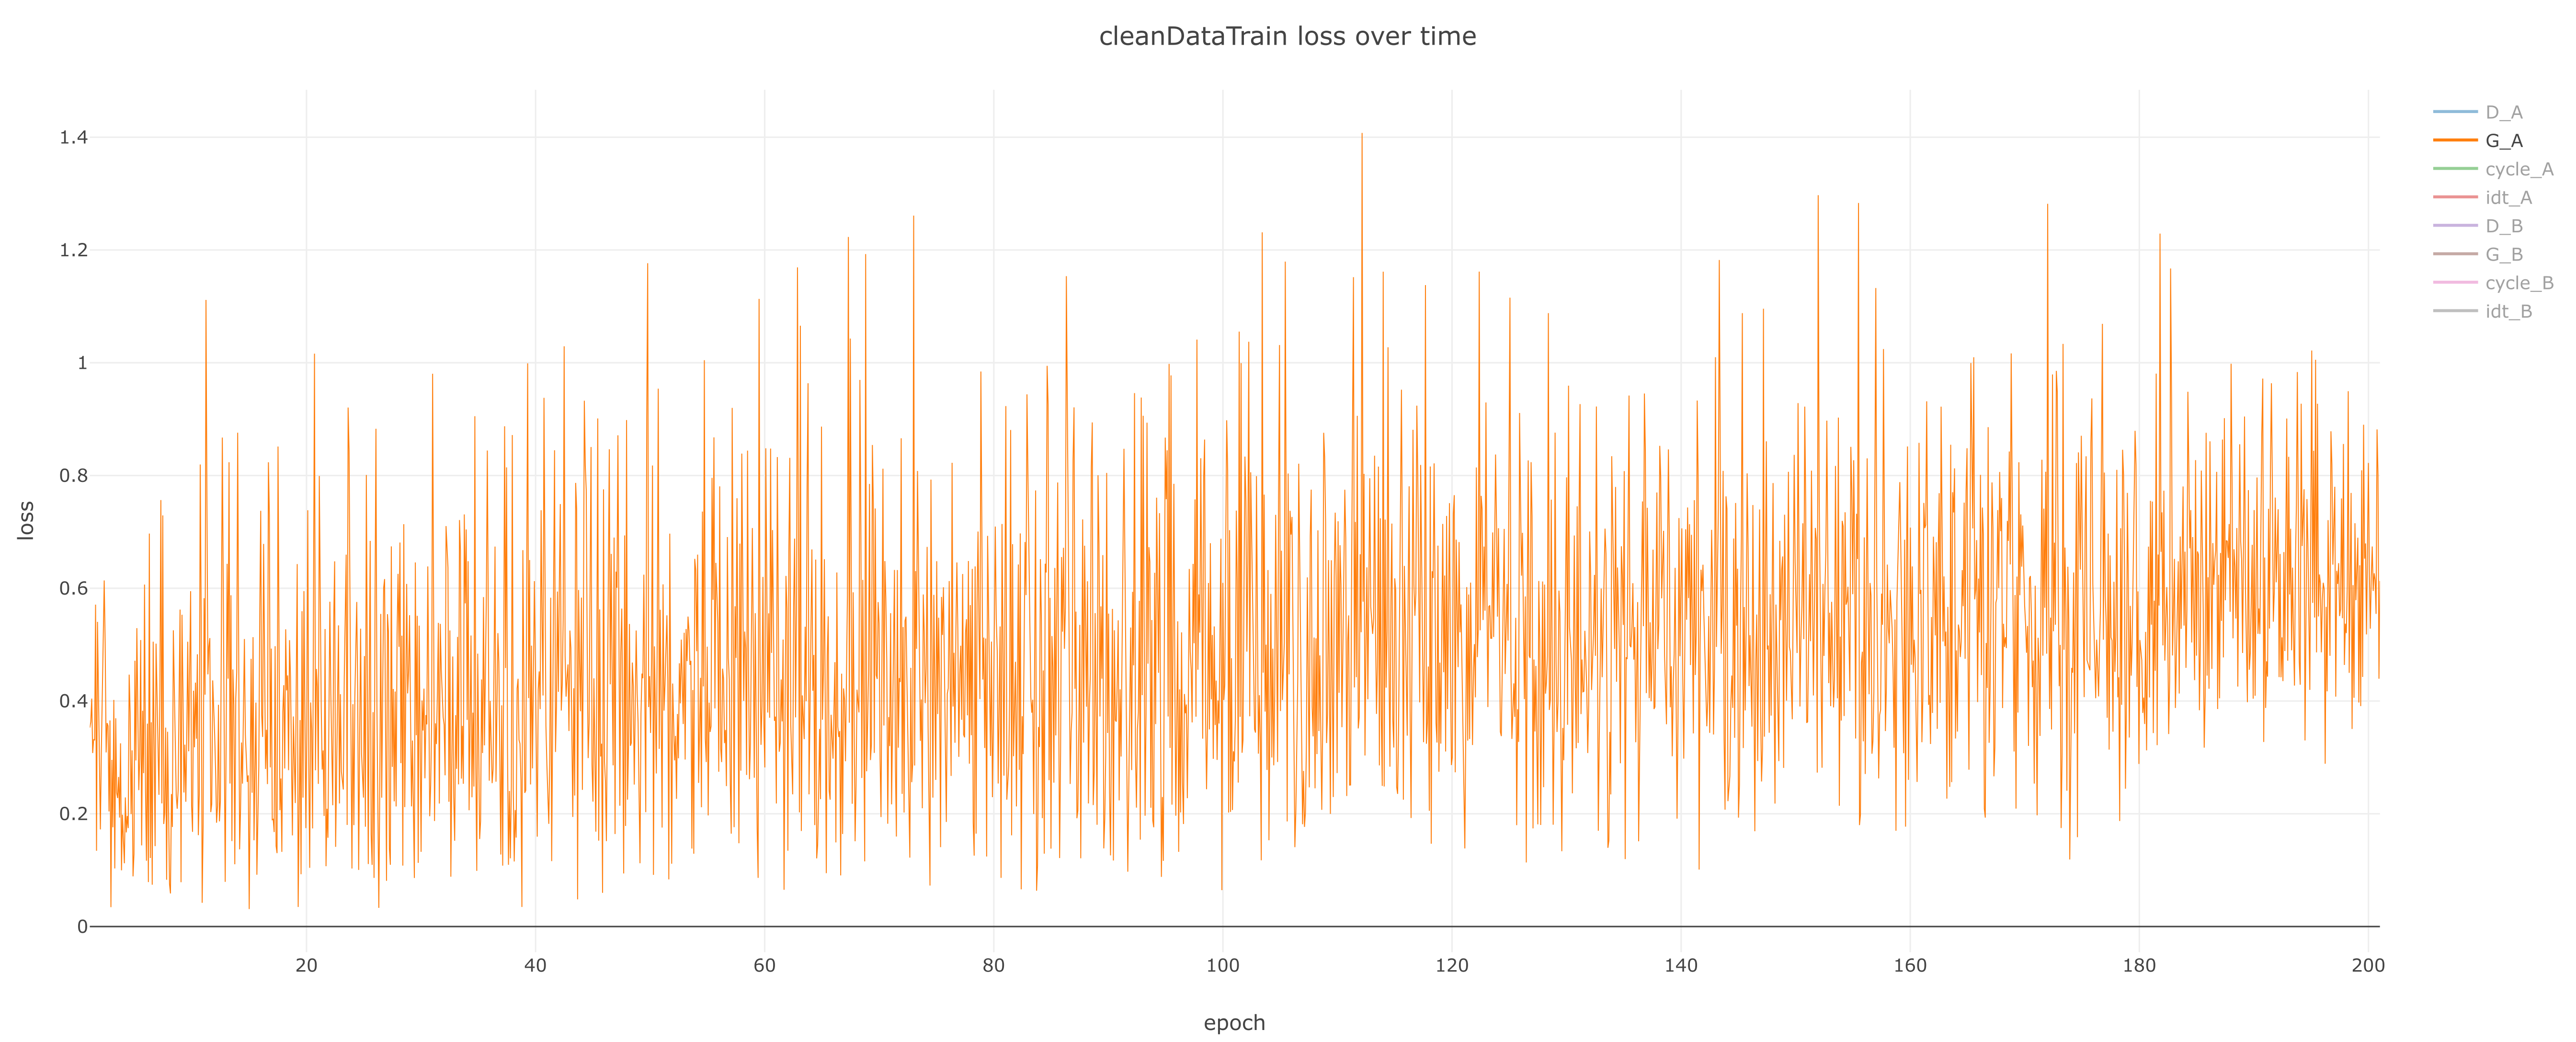
\includegraphics[width=1\textwidth]{chapter/losses_png/g_a.png}
    \caption{Adversarial (BCE) Loss for Color Generator}
     \end{figure}
    \pagebreak
    \newpage
    \begin{figure}[htbp]
    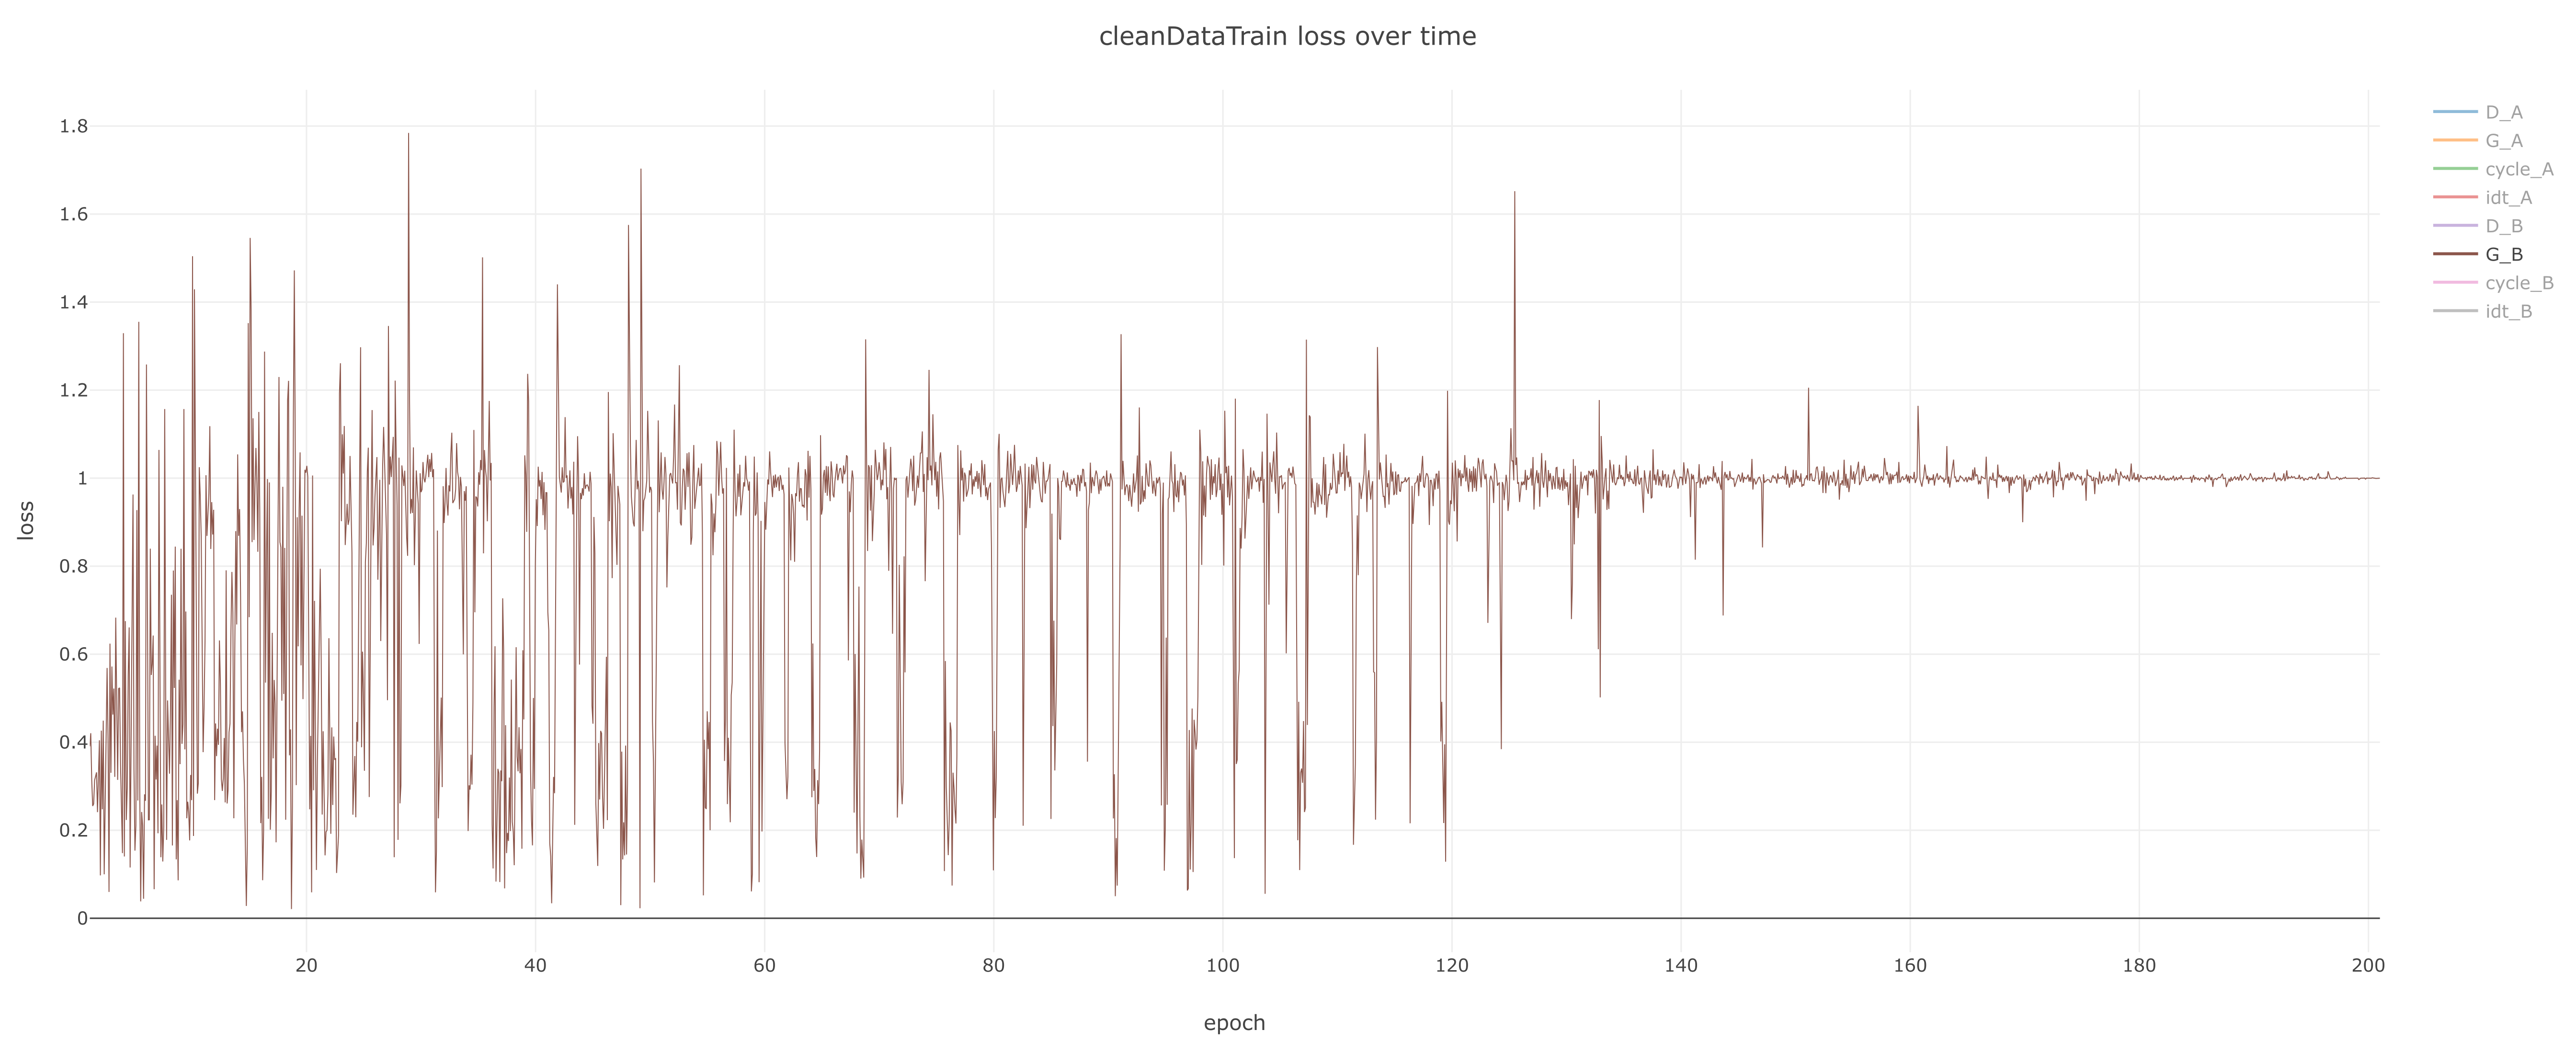
\includegraphics[width=1\textwidth]{chapter/losses_png/g_b.png}
    \caption{ Adversarial (BCE) Loss for BW Generator}
    
    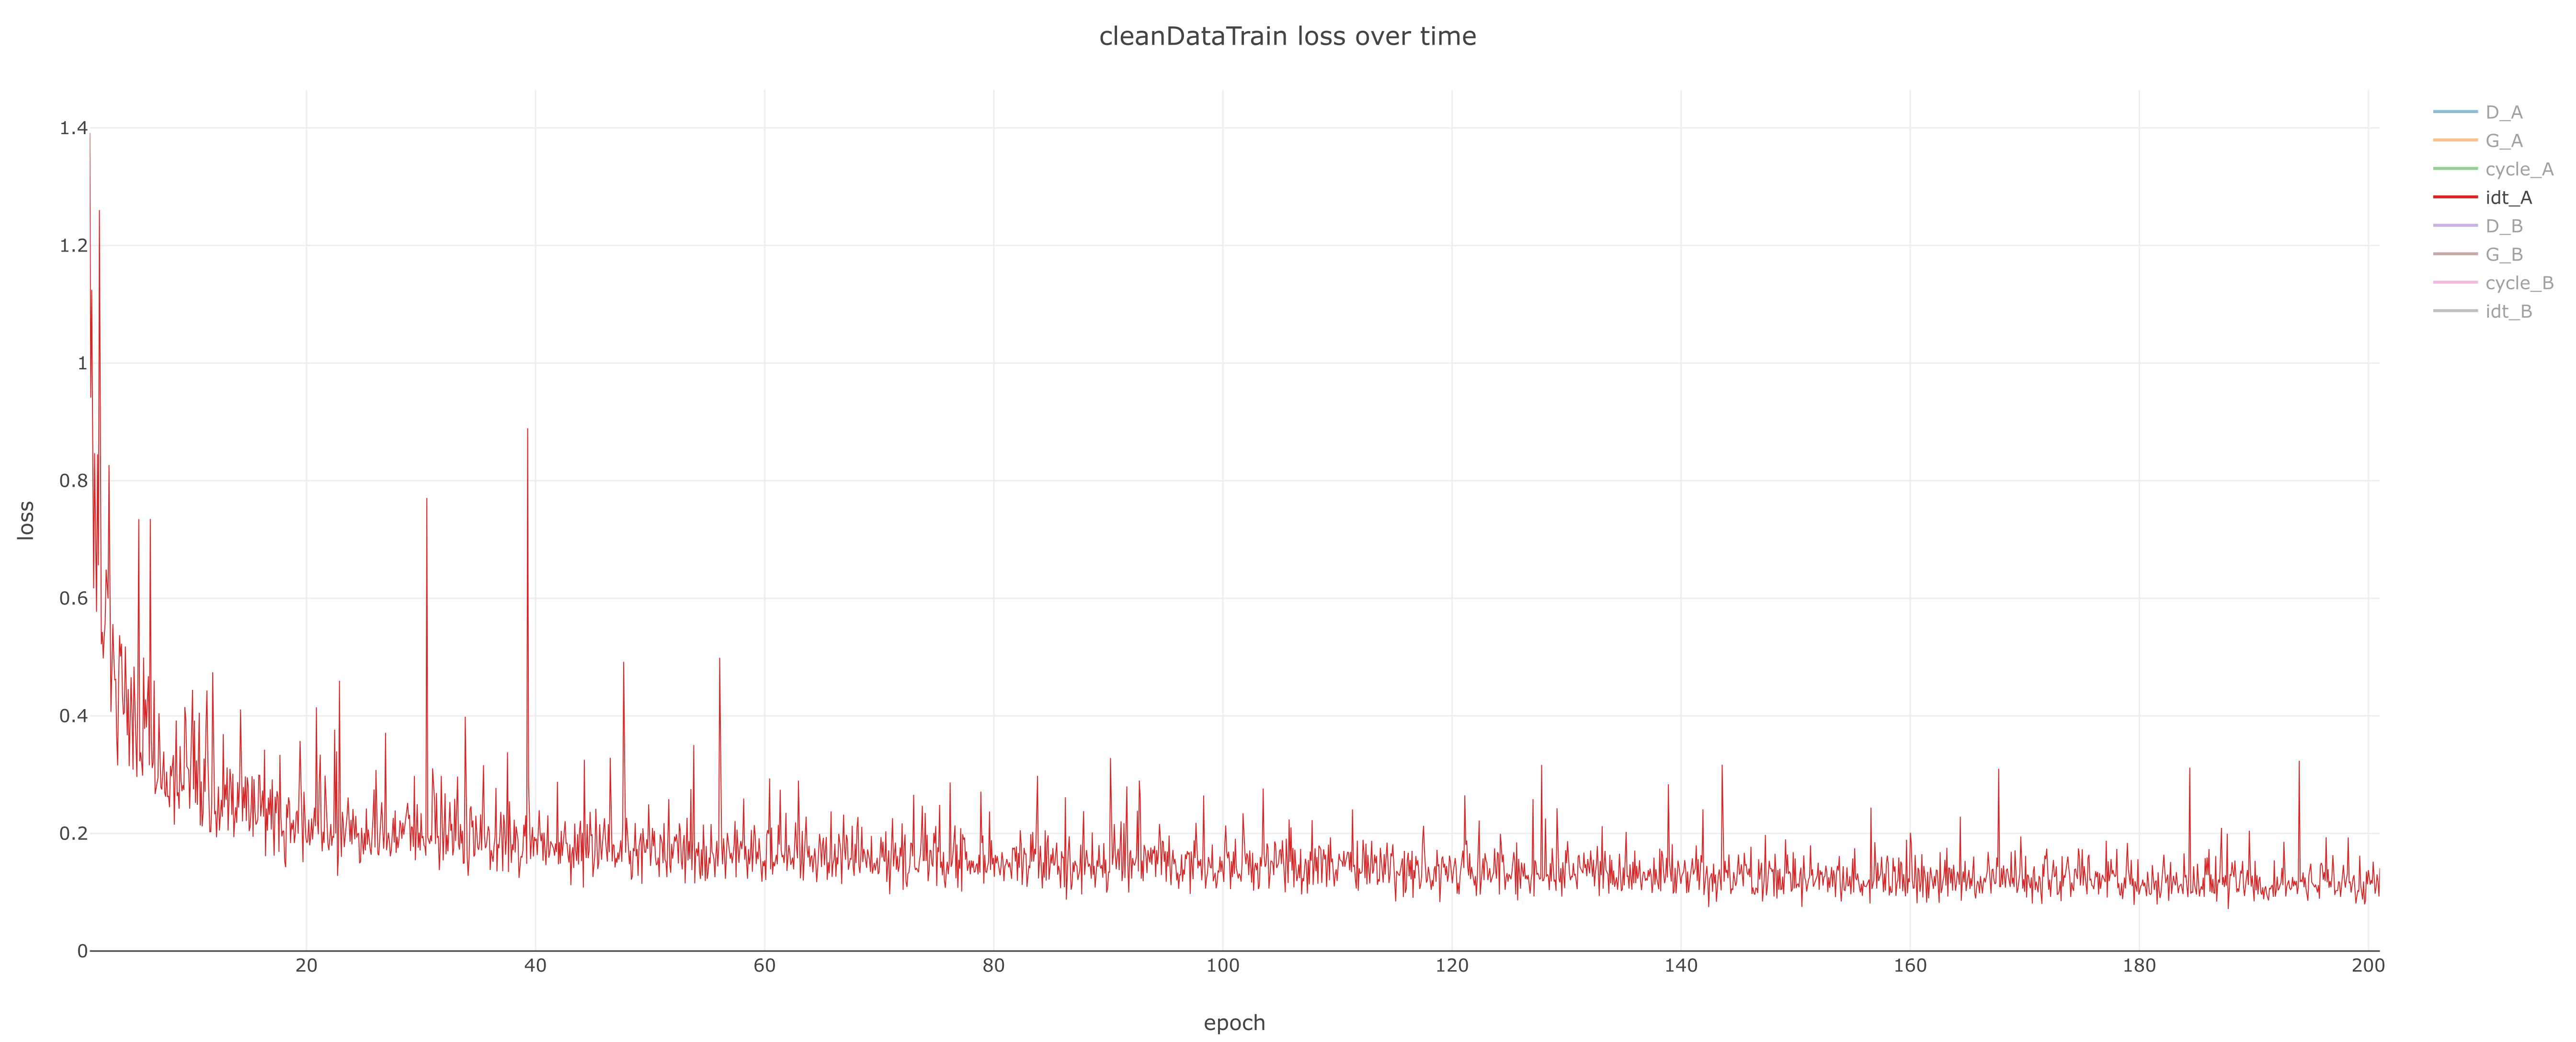
\includegraphics[width=1\textwidth]{chapter/losses_png/id_a.png}
    \caption{ Identity (L1) Loss for Color Generator}
    
    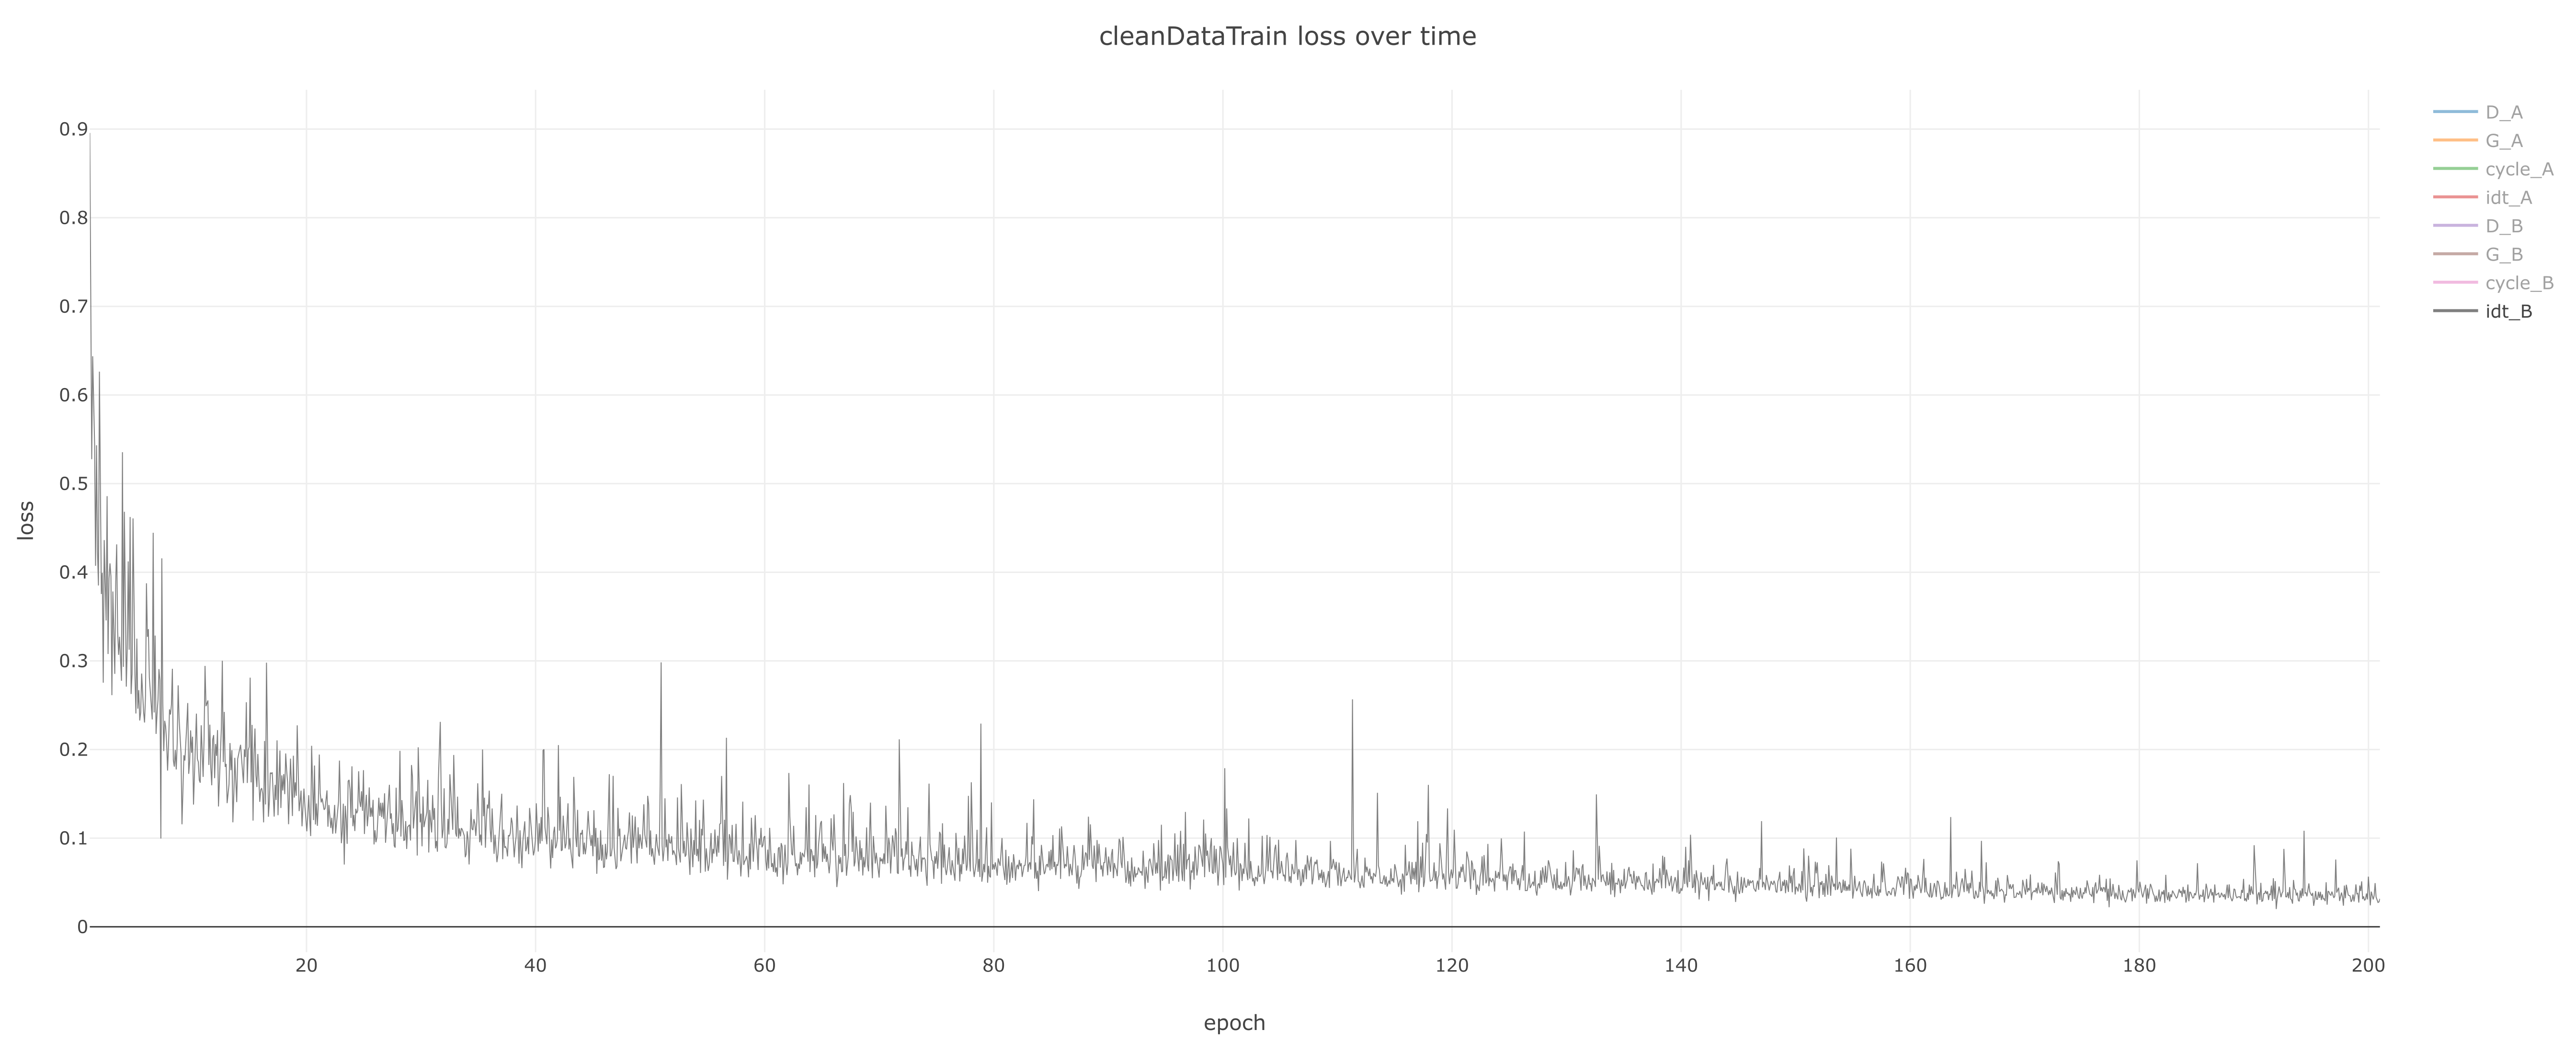
\includegraphics[width=1\textwidth]{chapter/losses_png/idt_b.png}
    \caption{ Identity (L2) Loss for Color Generator}

    \label{fig:enter-label}
\end{figure}